\chapter{Rezultati}\label{sec:rezultati}
Vse modele energijske porabe in srčnega utripa smo validirali na predhodno opisanih testnih vzorcih. Za primerjavo med različnimi modeli smo izbrali validacijske metrike: korelacijski koeficient (CORR), relativna absolutna napaka (RAE) in koren relativne kvadratne napake (RRSE) \cite{witten2005data}. Dodali smo tudi razmerje med številom podpornih vektorjev in številom učnih vzorcev (nSV). Višja je vrednost CORR predstavlja boljši rezultat, z RAE, RRSE in nSV pa je ravno obratno.

Modele smo ovrednotili tudi z navzkrižnim testiranjem. Testiranje je bilo opravljeno za stranski ali hrbtni pogled. \textit{sv} modeli, ki smo jih izdelali z učnimi vzorci iz stranske kamere, smo najprej preizkusili z učnimi vzorce iz stranske kamere in nato z vzorci iz hrbtne kamere. Navzkrižni testi imajo v oklepajih določen tip kamere, ki smo ga uporabili za vhodne podatke pri testiranju.
















\section{Eksperimenti 1. faze}


\subsection{Preliminarni testi}

\subsubsection{Optimizacija HOOF deskriptorjev}\label{sec:rezultati-optimizacija-hoof}
Parameter $N_{HOOF}$ smo določili na podlagi rezultatov evaluacije v tabeli \ref{tab:nhoof} in grafov korelacije med referenčnimi podatki in predikcijo \ref{fig:corr-hoof}.

V tabeli \ref{tab:nhoof} lahko vidimo, da se povečevanjem števila stolpcev rezultati bistveno ne razlikujejo. Najboljše rezultate nam sicer daje $120$ stolpcev, vendar pa smo za potrebe naše metode uporabili $N_{HOOF}=60$, ki je ravno tako dal zadovoljive rezultate. S takim številom smo zagotovili dobro delovanje glede na minimalno vrednost, še vseeno pa ne gre za tako veliko število, ko bi do izraza prišle amplitude šumnih vektorjev.

\begin{table}[!htbp]
	\centering
	\begin{tabular}{S[table-format=2.0] S[table-format=1.3] S[table-format=1.3] S[table-format=1.3] S[table-format=2.2]}
		\toprule
		\thead{$\mathbf{N_{HOOF}}$} & \thead{$\mathbf{r}$} & \thead{RAE} & \thead{RRSE} & \thead{nSV [\%]}\\
		\midrule%nSV
		30 & 0.978 & 0.296 & 0.304 & \boldentry{2}{2}{62.81}\\%18089
		\boldentry{2}{0}{60} & 0.980 & 0.277 & 0.289 & 81.21\\%23388
		120 & \boldentry{1}{2}{0.983} & \boldentry{1}{3}{0.261} & \boldentry{1}{3}{0.273} & 74.39\\%21424
		160 & 0.982 & 0.272 & 0.284 & 71.68\\%20644
		\bottomrule
	\end{tabular}
	\caption[Rezultati evaluacije modelov z različnim $N_{HOOF}$]{Rezultati evaluacije modelov z različnim številom stolpcev $N_{HOOF}$ HOOF deskriptorja. Optimalni rezultati so odebeljeni. Kljub dobrim rezultatom modela z $N_{HOOF}=120$ smo izbrali $N_{HOOF}=60$, ker nanj šum manj vpliva.}
	\label{tab:nhoof}
\end{table}

\begin{figure}[!htbp]
	\centering
	\begin{subfigure}[t]{0.45\columnwidth}
		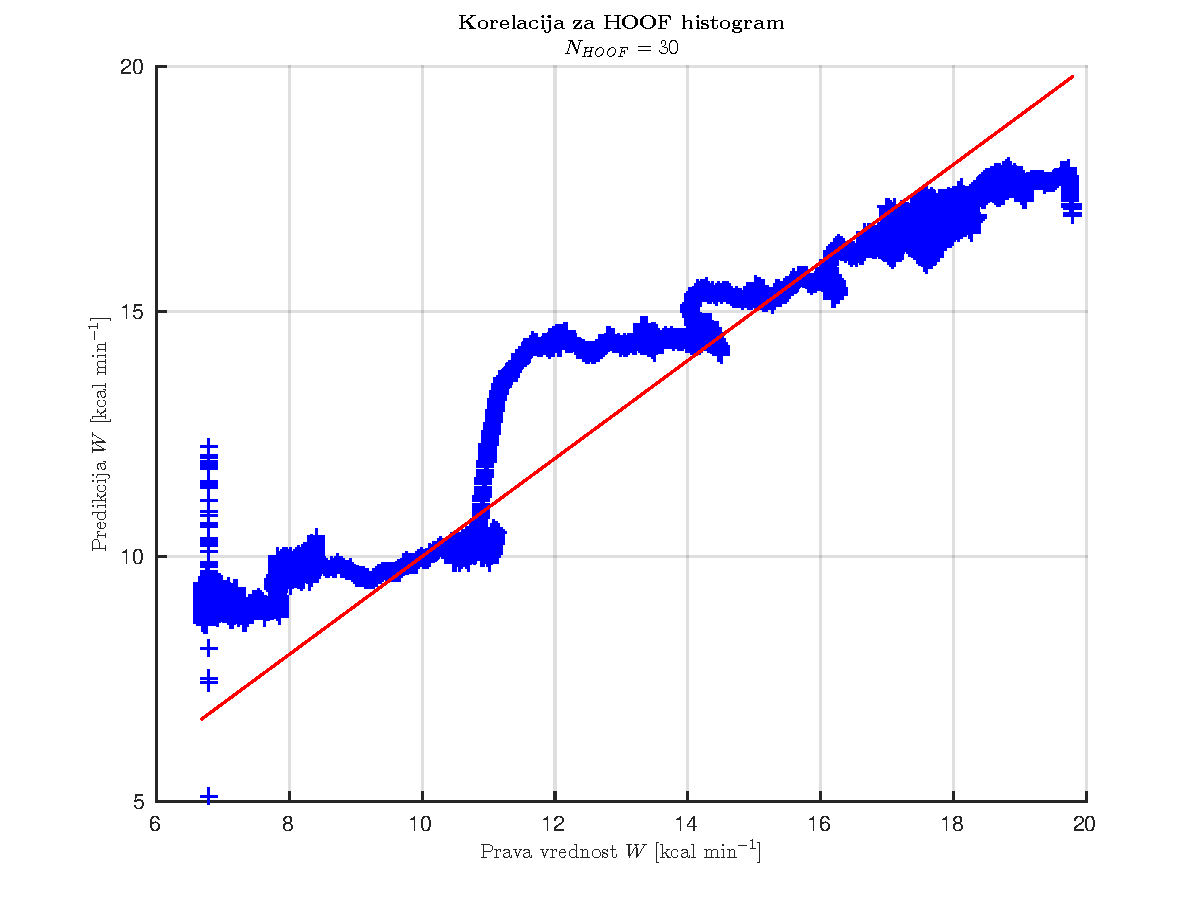
\includegraphics[width=\columnwidth]{corr-hoof-30-sl}
		\caption{Korelacija $N_{HOOF}=30$.}
		\label{fig:corr-hoof-30}
	\end{subfigure}
	~
	\begin{subfigure}[t]{0.45\columnwidth}
		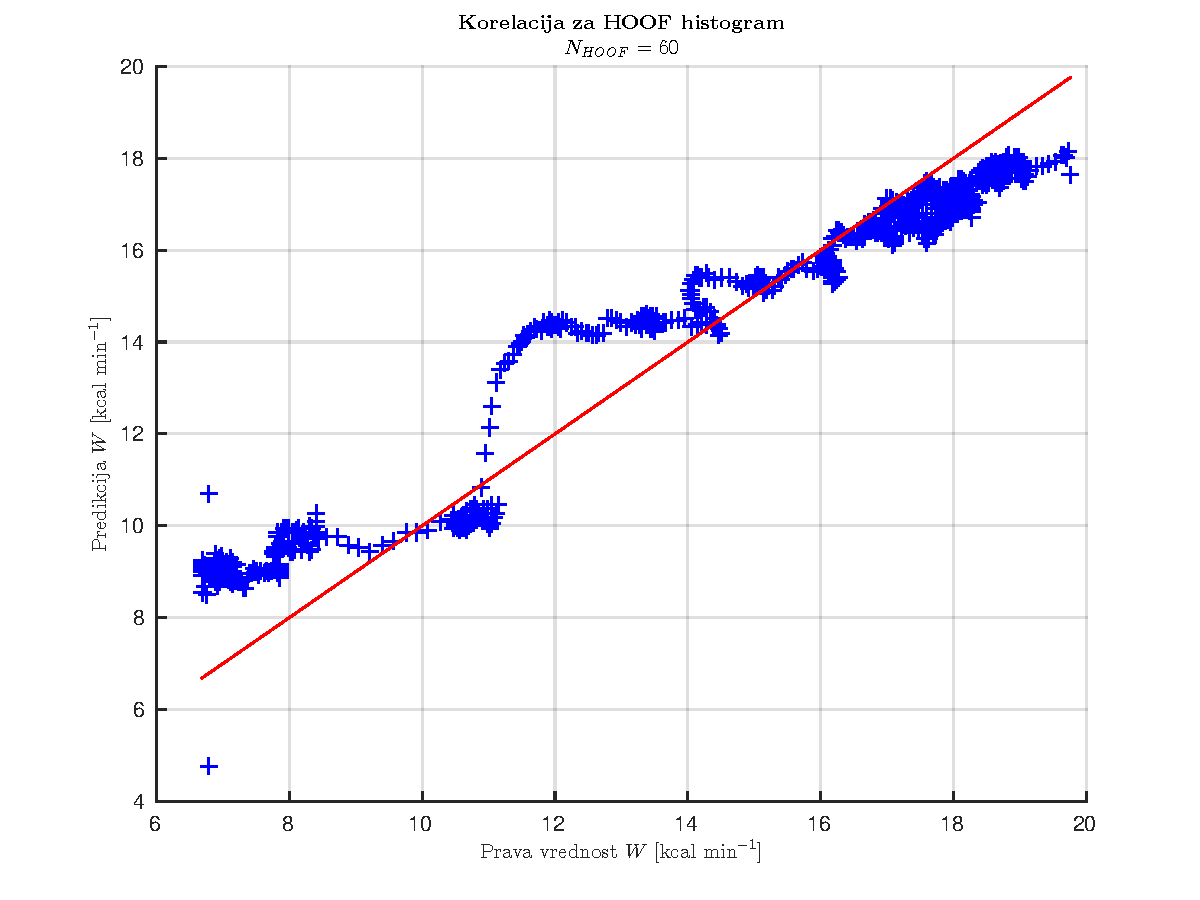
\includegraphics[width=\columnwidth]{corr-hoof-60-sl}
		\caption{Korelacija $N_{HOOF}=60$.}
		\label{fig:corr-hoof-60}
	\end{subfigure}
	~
	\begin{subfigure}[b]{0.45\columnwidth}
		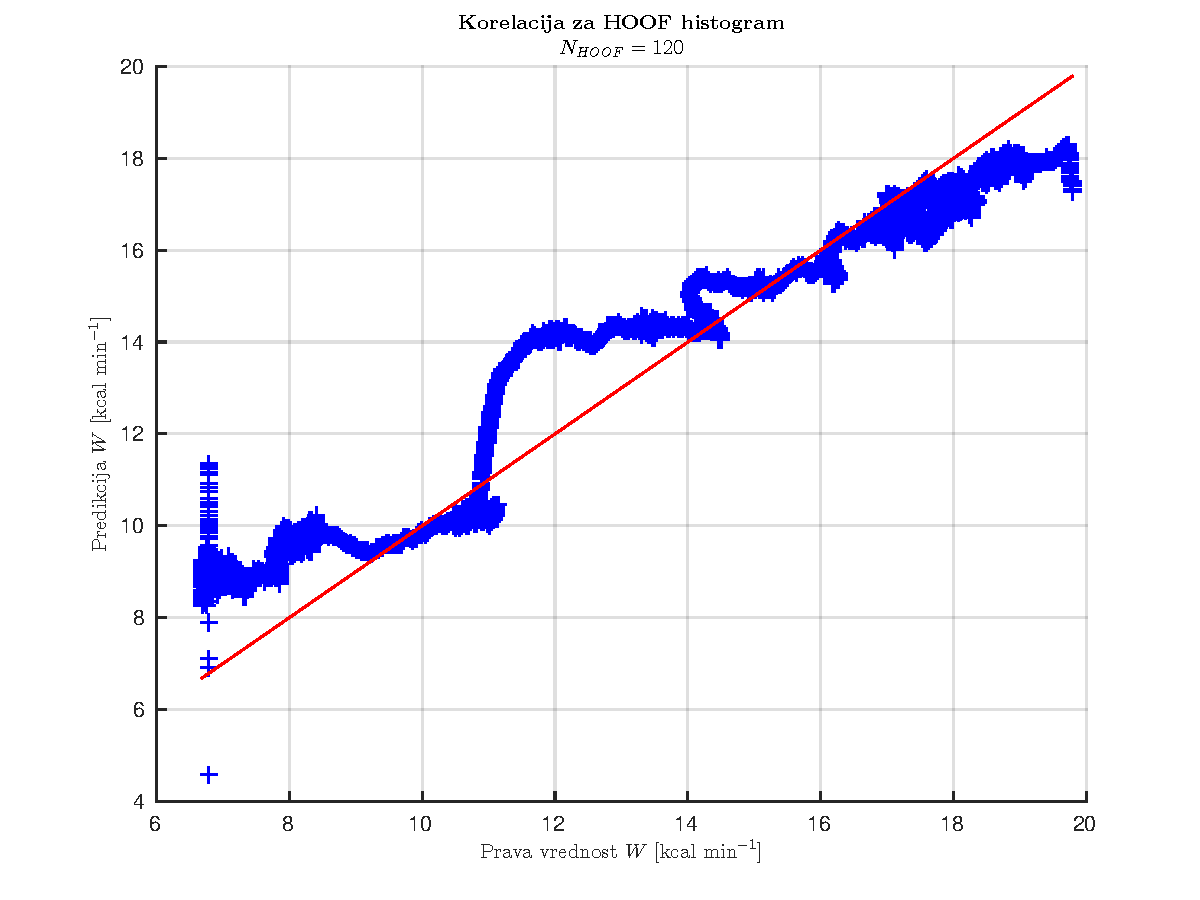
\includegraphics[width=\columnwidth]{corr-hoof-120-sl}
		\caption{Korelacija $N_{HOOF}=120$.}
		\label{fig:corr-hoof-120}
	\end{subfigure}
	~
	\begin{subfigure}[b]{0.45\columnwidth}
		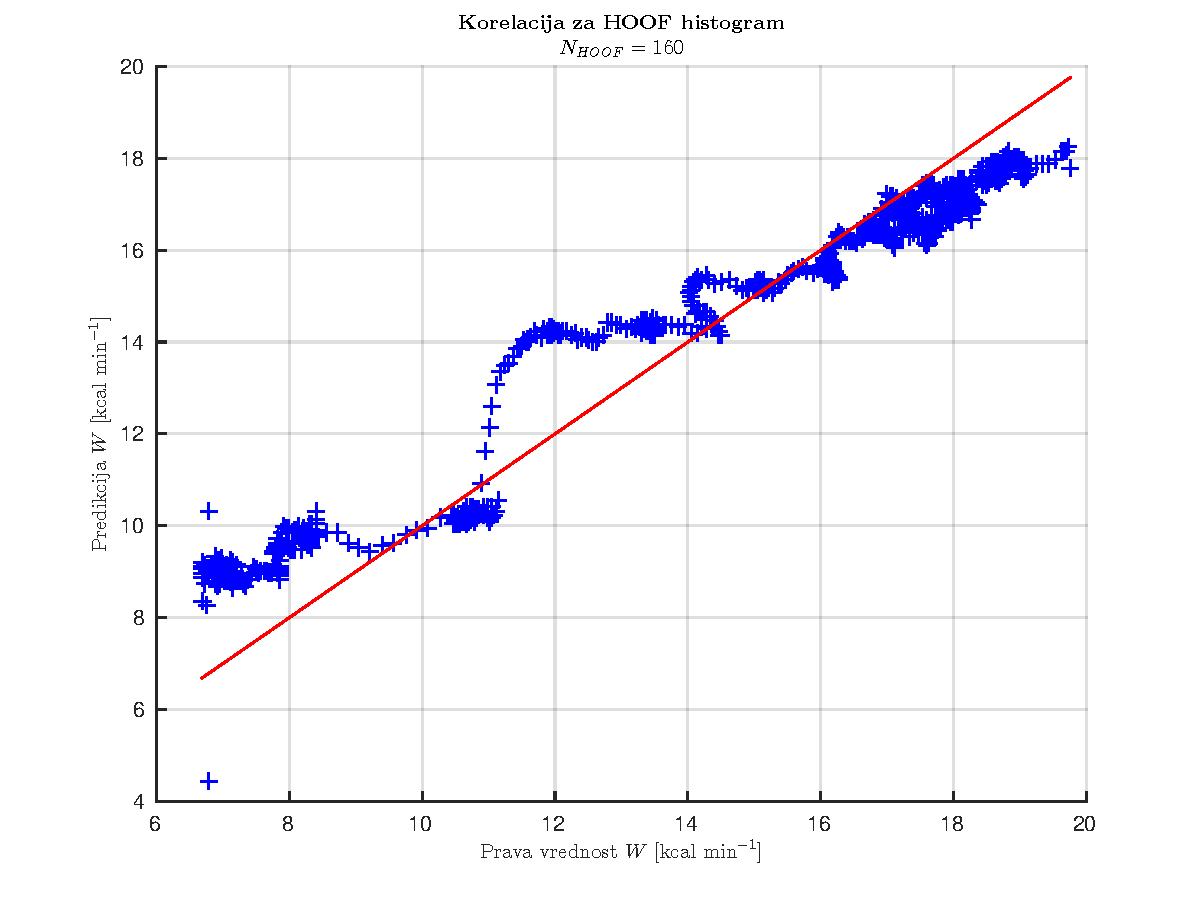
\includegraphics[width=\columnwidth]{corr-hoof-160-sl}
		\caption{Korelacija $N_{HOOF}=160$.}
		\label{fig:corr-hoof-160}
	\end{subfigure}
	\caption[Grafi korelacij modelov z različnim $N_{HOOF}$]{Grafi korelacij modelov z različnim številom stolpcev $N_{HOOF}$ HOOF deskriptorja. Rezultati so si zelo podobni.}
	\label{fig:corr-hoof}
\end{figure}












\subsubsection{Optimizacija HAFA deskriptorjev}\label{sec:rezultati-optimizacija-hafa}
Parameter $N_{HAFA}$ smo določili na podlagi rezultatov evaluacije v tabeli \ref{tab:nhafa} in grafov korelacije med referenčnimi podatki in predikcijo \ref{fig:corr-hafa}.

\begin{table}[!htbp]
	\centering
	\begin{tabular}{S[table-format=2.0] S[table-format=1.3] S[table-format=1.3] S[table-format=1.3] S[table-format=2.2]}
		\toprule
		\thead{$\mathbf{N_{HAFA}}$} & \thead{$\mathbf{r}$} & \thead{RAE} & \thead{RRSE} & \thead{nSV [\%]}\\
		\midrule%nSV
		30 & 0.984 & 0.213 & 0.231 & 62.08 \\%17879/28799
		\boldentry{2}{0}{60} & \boldentry{1}{3}{0.984} & \boldentry{1}{3}{0.211} & \boldentry{1}{3}{0.228} & \boldentry{2}{2}{62.60} \\%18028
		120 & 0.984 & 0.211 & 0.228 & 62.63 \\%18037
		160 & 0.984 & 0.211 & 0.228 & 62.63 \\%18037
		\bottomrule
	\end{tabular}
	\caption[Rezultati evaluacije modelov z različnim $N_{HAFA}$]{Rezultati evaluacije modelov z različnim številom stolpcev $N_{HAFA}$ HAFA deskriptorja. Optimalni rezultati so odebeljeni.}
	\label{tab:nhafa}
\end{table}

V tabeli \ref{tab:nhafa} lahko vidimo, da so rezultati praktično enaki. Za našo metodo smo izbrali $N_{HAFA}=60$, kar v grobem predstavlja $60$ različnih hitrosti z maksimalno amplitudo \SI{60}{px.f^{-1}}.

\begin{figure}[!htbp]
	\centering
	\begin{subfigure}[t]{0.45\columnwidth}
		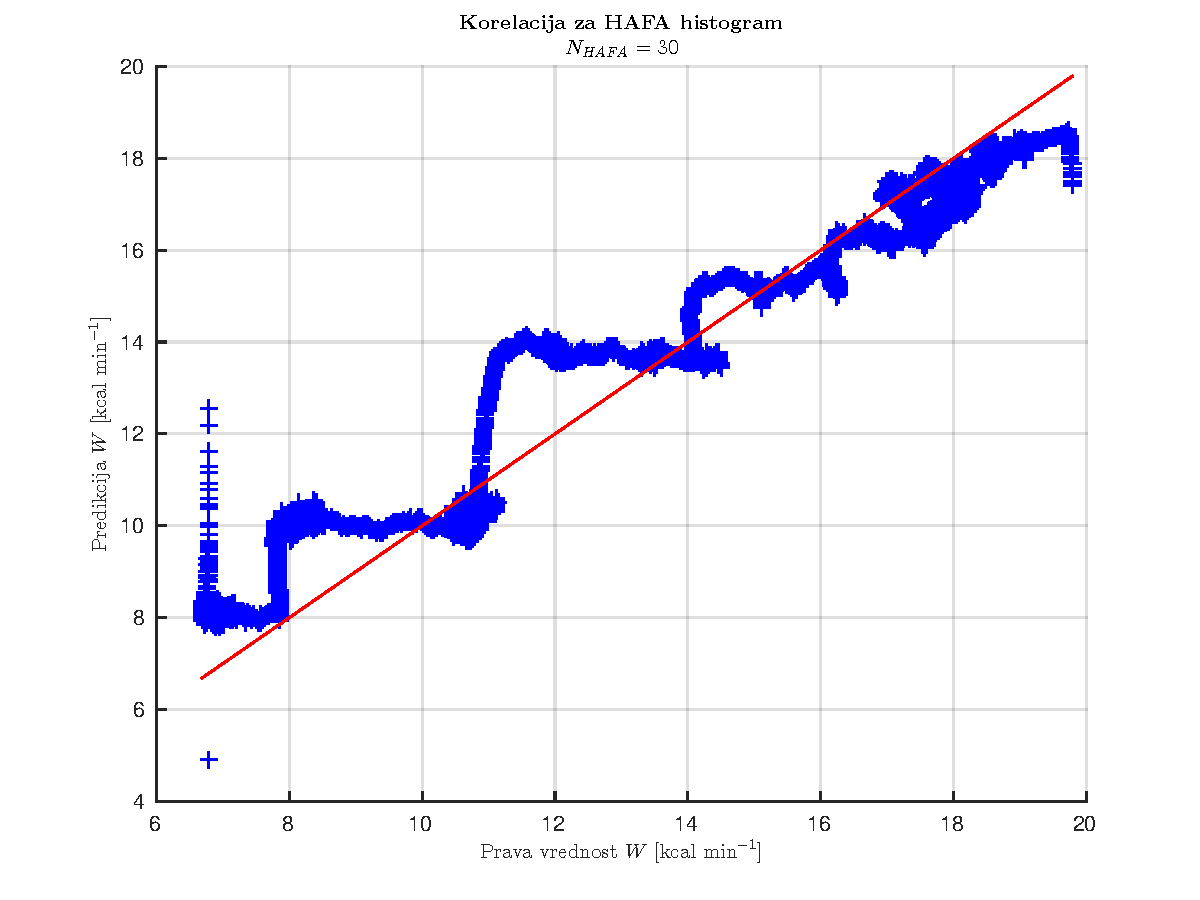
\includegraphics[width=\columnwidth]{corr-hafa-30-sl}
		\caption{Korelacija $N_{HAFA}=30$.}
		\label{fig:corr-hafa-30}
	\end{subfigure}
	~
	\begin{subfigure}[t]{0.45\columnwidth}
		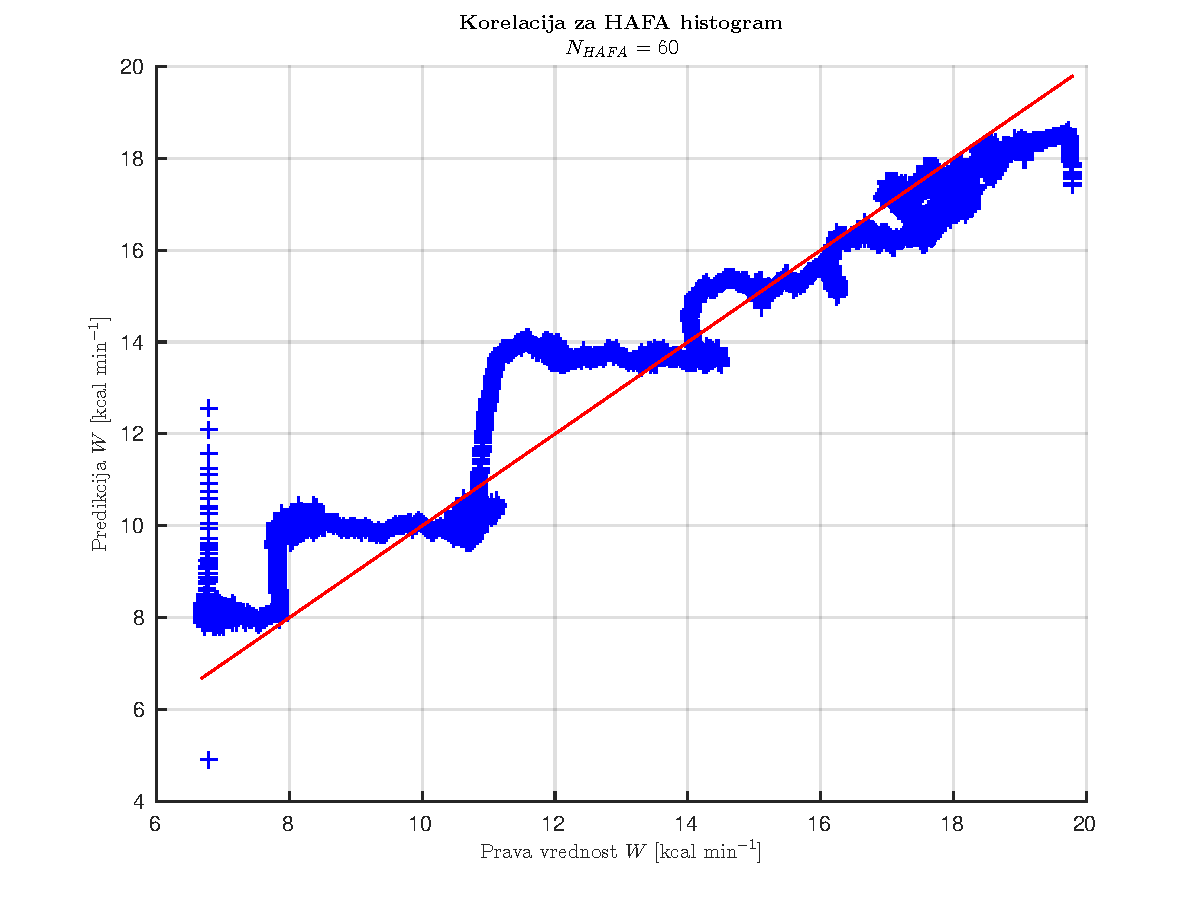
\includegraphics[width=\columnwidth]{corr-hafa-60-sl}
		\caption{Korelacija $N_{HAFA}=60$.}
		\label{fig:corr-hafa-60}
	\end{subfigure}
	~
	\begin{subfigure}[b]{0.45\columnwidth}
		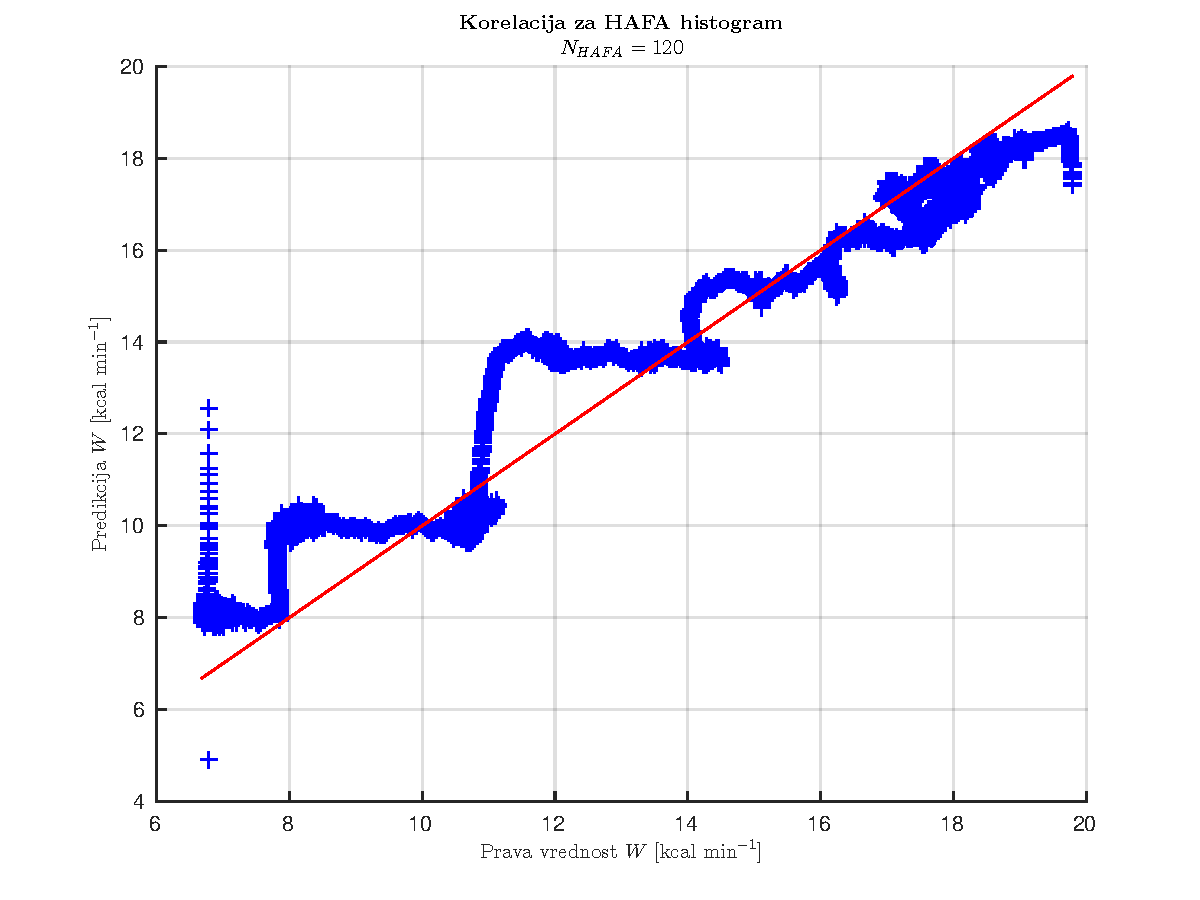
\includegraphics[width=\columnwidth]{corr-hafa-120-sl}
		\caption{Korelacija $N_{HAFA}=120$.}
		\label{fig:corr-hafa-120}
	\end{subfigure}
	~
	\begin{subfigure}[b]{0.45\columnwidth}
		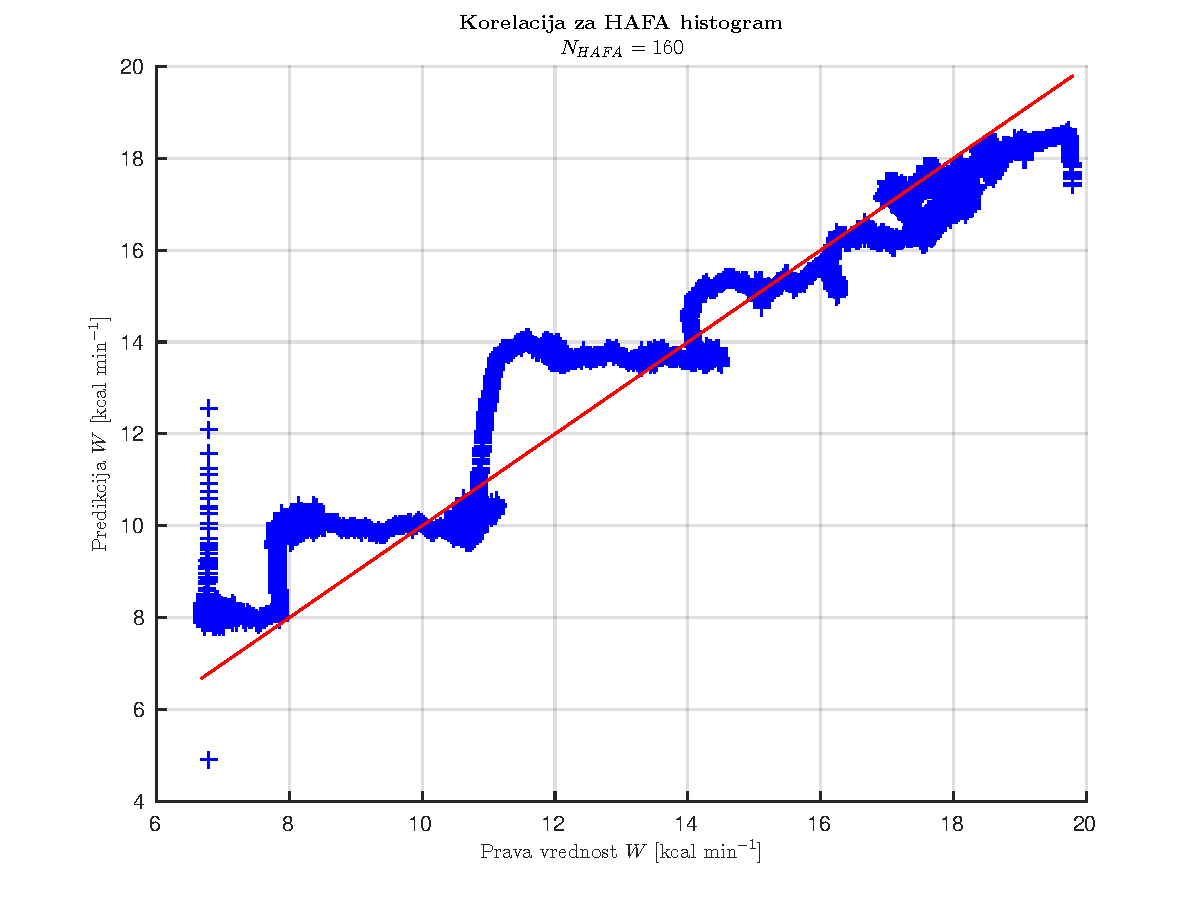
\includegraphics[width=\columnwidth]{corr-hafa-160-sl}
		\caption{Korelacija $N_{HAFA}=160$.}
		\label{fig:corr-hafa-160}
	\end{subfigure}
	\caption[Grafi korelacij modelov z različnim $N_{HAFA}$]{Grafi korelacij modelov z različnim številom stolpcev $N_{HAFA}$ HAFA deskriptorja. Rezultati so si zelo podobni.}
	\label{fig:corr-hafa}
\end{figure}











\subsubsection{Razširitev HOOF deskriptorja}\label{sec:rezultati-razsiritev-hoof}

\begin{table}[!htbp]
	\centering
	\begin{tabular}{l S[table-format=1.3] S[table-format=1.3] S[table-format=1.3] S[table-format=2.2]}
		\toprule
		\textbf{Deskriptor} & \thead{$\mathbf{r}$} & \thead{RAE} & \thead{RRSE} & \thead{nSV [\%]}\\
		\midrule%nSV
		HOOF & 0.992 & 0.336 & 0.317 & \boldentry{2}{2}{82.34} \\%2187/2656
		\textbf{HOOF-HAFA} & \boldentry{1}{3}{0.991} & \boldentry{1}{3}{0.157} & \boldentry{1}{3}{0.205} & 89.53 \\%2378
		\bottomrule
	\end{tabular}
	\caption[Rezultati evaluacije modelov z različnim deskriptorjem]{Rezultati evaluacije modelov z različnim deskriptorjem. Optimalni rezultati so odebeljeni. Vidimo lahko, da se bolje odnese razširjeni deskriptor HOOF-HAFA, čeprav model uporablja več podpornih vektorjev. }
	\label{tab:izbira}
\end{table}



\begin{figure}[!htbp]
	\centering
	\begin{subfigure}[t]{0.45\columnwidth}
		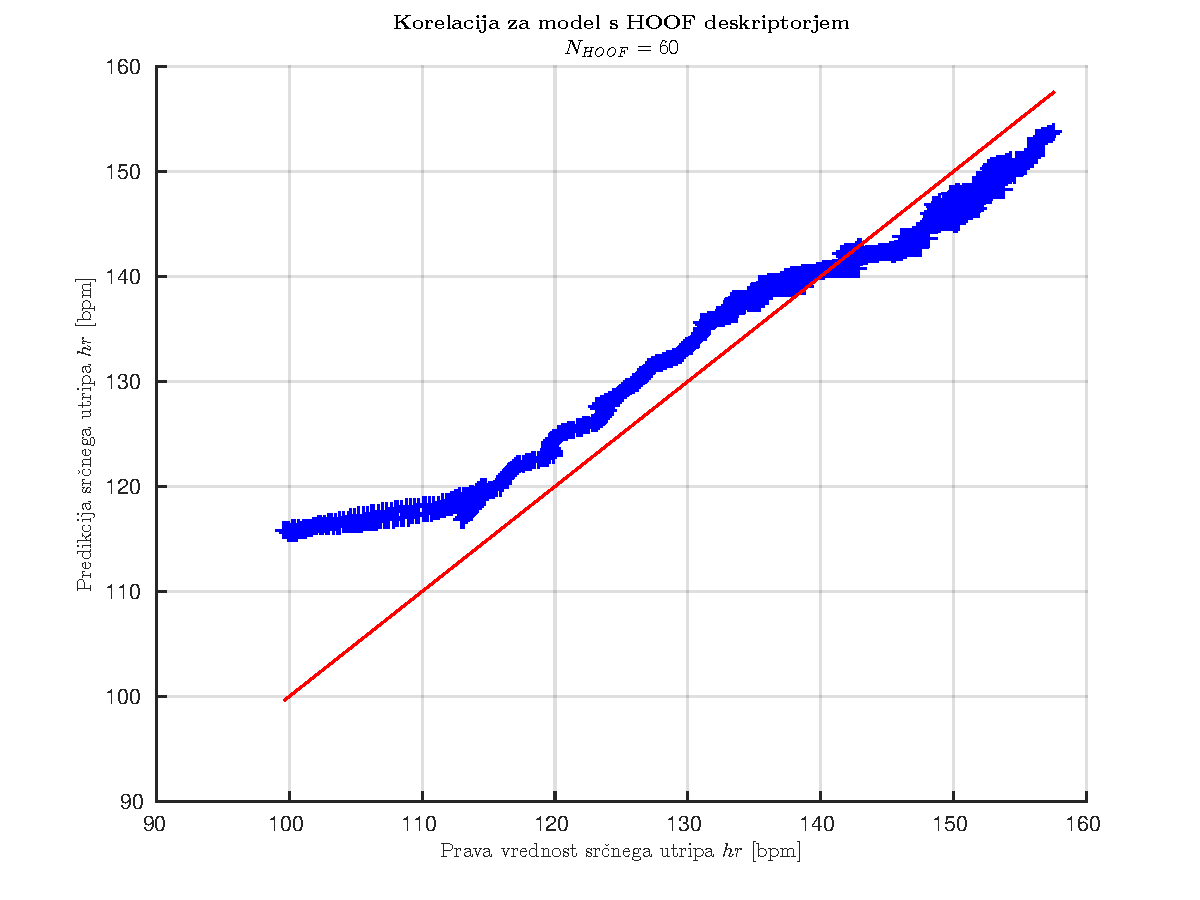
\includegraphics[width=\columnwidth]{corr-hoof-sl}
		\caption{Korelacija $N_{HOOF}=60$.}
		\label{fig:izbira-hoof}
	\end{subfigure}
	~
	\begin{subfigure}[t]{0.45\columnwidth}
		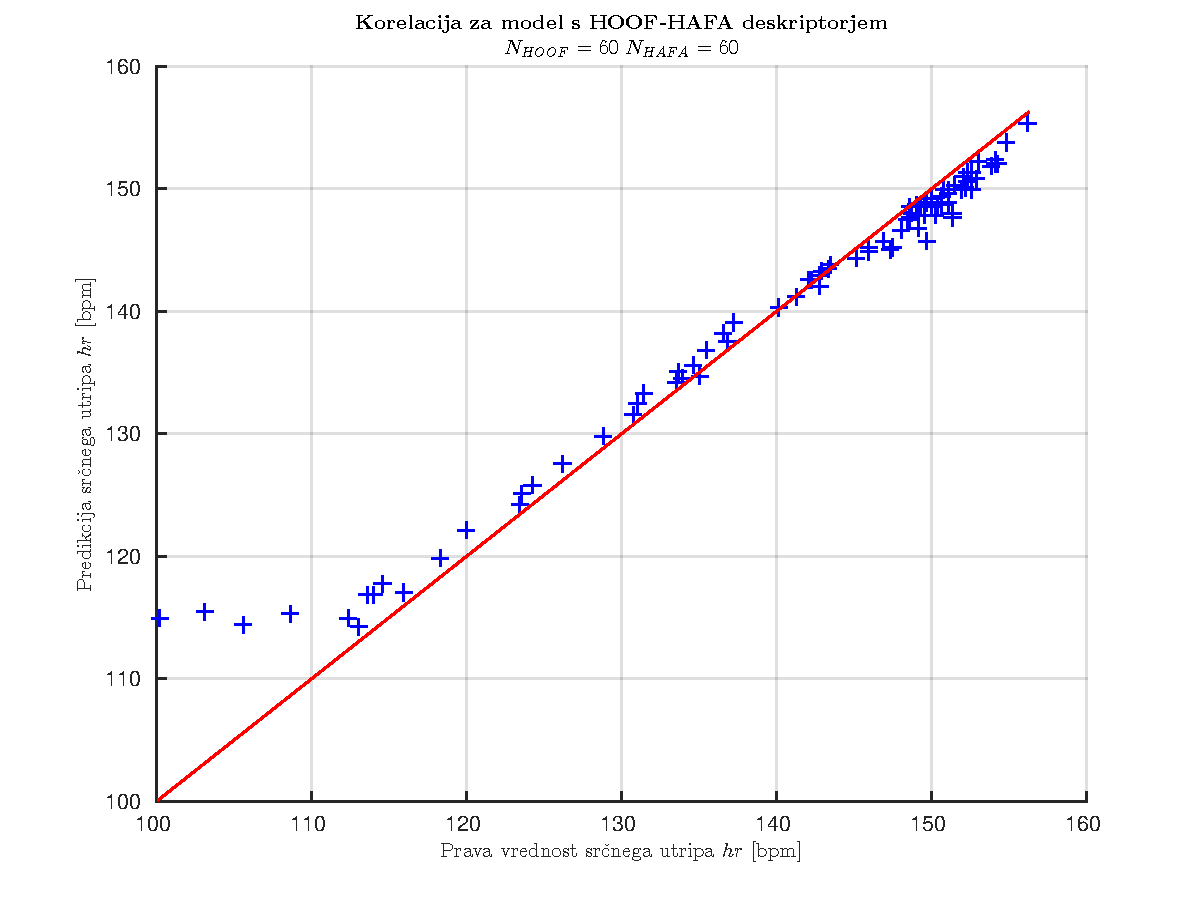
\includegraphics[width=\columnwidth]{corr-hoof-hafa-sl}
		\caption{Korelacija $N_{HOOF}=60$,\\$N_{HAFA}=60$.}
		\label{fig:izbira-hoofhafa}
	\end{subfigure}
	\caption[Primerjava modelov s HOOF in HOOF-HAFA deskriptorji]{Primerjava grafov korelacij modelov z različnimi deskriptorji. Model \subref{fig:izbira-hoof}) smo naučili s HOOF deskriptorjem. Model \subref{fig:izbira-hoofhafa}) smo naučili s HOOF in HAFA deskriptorjem. Posamezen vzorec je tako vseboval $120$ značilk. Pri primerjavi korelacije lahko opazimo vidno razliko. Model \subref{fig:izbira-hoofhafa}) dokazuje, da je razširjeni deskriptor boljši.}
	\label{fig:izbira}
\end{figure}




















\subsubsection{Sledilniki za optični tok} \label{sec:rezultati-sledilnikov-za-opticni-tok}


Rezultati testiranja so prikazani v tabeli \ref{tab:region-overlap}. Za izbrane sledilnike smo določili povprečje prekrivanja področja za posamezen posnetek. V tretjem stolpcu je predstavljeno povprečje prekrivanja glede na oba posnetka. Najboljši rezultati so odebeljeni. Po tabeli \ref{tab:region-overlap} se za posnetek \textit{handball1} najbolje izkaže CORR sledilnik. Za posnetek \textit{handball2} smo dobili najboljše rezultate pri sledilniku OPENCV-TLD. V povprečju se najbolje izkaže sledilnik CORR.




\begin{table}[!htbp]
	\centering
	\begin{tabular}{l S[table-format=1.3] S[table-format=1.3] S[table-format=1.3]}
		\toprule
		\textbf{Sledilnik} & \thead{$\mathbf{\Phi(\mathrm{handball1})}$} & \thead{$\mathbf{\Phi(\mathrm{handball2})}$} & \thead{$\mathbf{\overline{\Phi}}$}  \\
		\midrule%nSV
		NEBEHAY-TLD & 0.035 & 0.130 & 0.083 \\
		CCV-TLD & 0.117 & 0 & 0.117 \\
		OPENCV-TLD & 0.002 & \boldentry{1}{3}{0.178} & 0.09 \\
		CORR & \boldentry{1}{3}{0.214} & 0.160 & \boldentry{1}{3}{0.187} \\
		\textbf{KCF} & {0.161} & {0.166} & {0.164} \\
		\bottomrule
	\end{tabular}
	\caption[Povprečje prekrivanja področja za posamezen sledilnik]{Povprečje prekrivanja področja za posamezen sledilnik in posnetek. V tretjem stolpcu je predstavljeno povprečje prekrivanja glede na oba posnetka. Najboljši rezultati so odebeljeni. Po tabeli \ref{tab:region-overlap} se za posnetek \textit{handball1} najbolje izkaže CORR sledilnik. Za posnetek \textit{handball2} smo dobili najboljše rezultate pri sledilniku OPENCV-TLD. V povprečju se najbolje izkaže sledilnik CORR.}
	\label{tab:region-overlap}
\end{table}


Na sliki \ref{fig:tracker-visual} lahko vidimo primer delovanja sledilnikov za oba posnetka. Referenčni igralec, ki mu morajo slediti ima rumeno majico. Za posnetek \textit{handball1} je predstavljena 15. slika, za posnetek \textit{handball2} pa 111. slika. Rezultati v tabeli \ref{tab:region-overlap} se skladajo z opažanji na sliki \ref{fig:tracker-visual}.

\begin{figure}[!htbp]
	\centering	
	\begin{subfigure}[t]{0.45\columnwidth}
		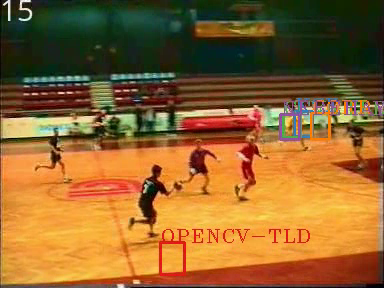
\includegraphics[width=\columnwidth]{handball1-example.png}
		\caption{15. slika posnetka \textit{handball1}.}
		\label{fig:handball1}
	\end{subfigure}
	~
	\begin{subfigure}[t]{0.45\columnwidth}
		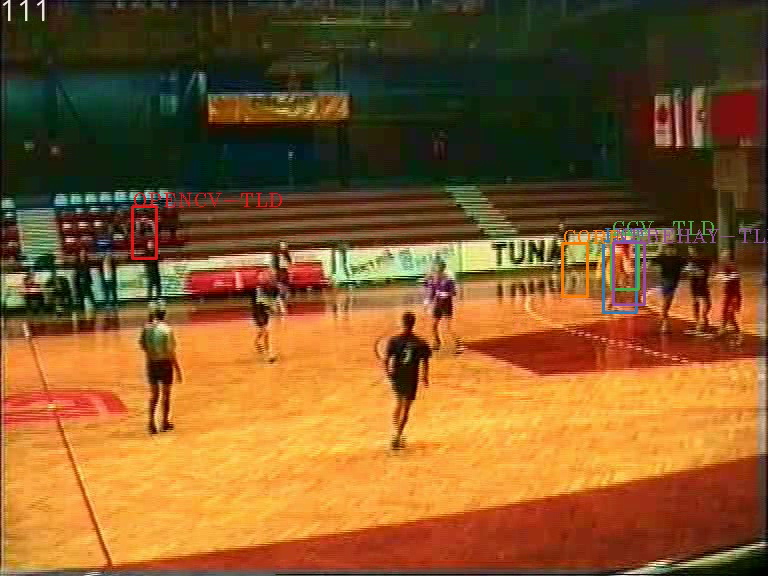
\includegraphics[width=\columnwidth]{/handball2-example.png}
		\caption{111. slika posnetka \textit{handball2}.}
		\label{fig:handball2}
	\end{subfigure}  
	\caption[Primer delovanja sledilnikov za \textit{handball} posnetke]{Primer delovanja sledilnikov za \textit{handball} posnetke. Referenčni igralec, ki mu morajo slediti ima rumeno majico. }
	\label{fig:tracker-visual}
\end{figure}




Čeprav smo z mero določili, da se je najbolje izkazal sledilnik CORR, se je pri hitri vizualni oceni sledenja na izsekih posnetka \cite{squashtv2014squash} izkazalo, da najbolje deluje sledilnik KCF. Primer boljšega delovanja KCF sledilnika je slika \ref{fig:squash-tracker-visual}, kjer sledimo modremu igralcu. Na isti sliki posnetka je KCF algoritem našel modrega igralca, medtem ko ga je CORR algoritem zamenjal z drugim igralcem. 



\begin{figure}[!htbp]
	\centering
	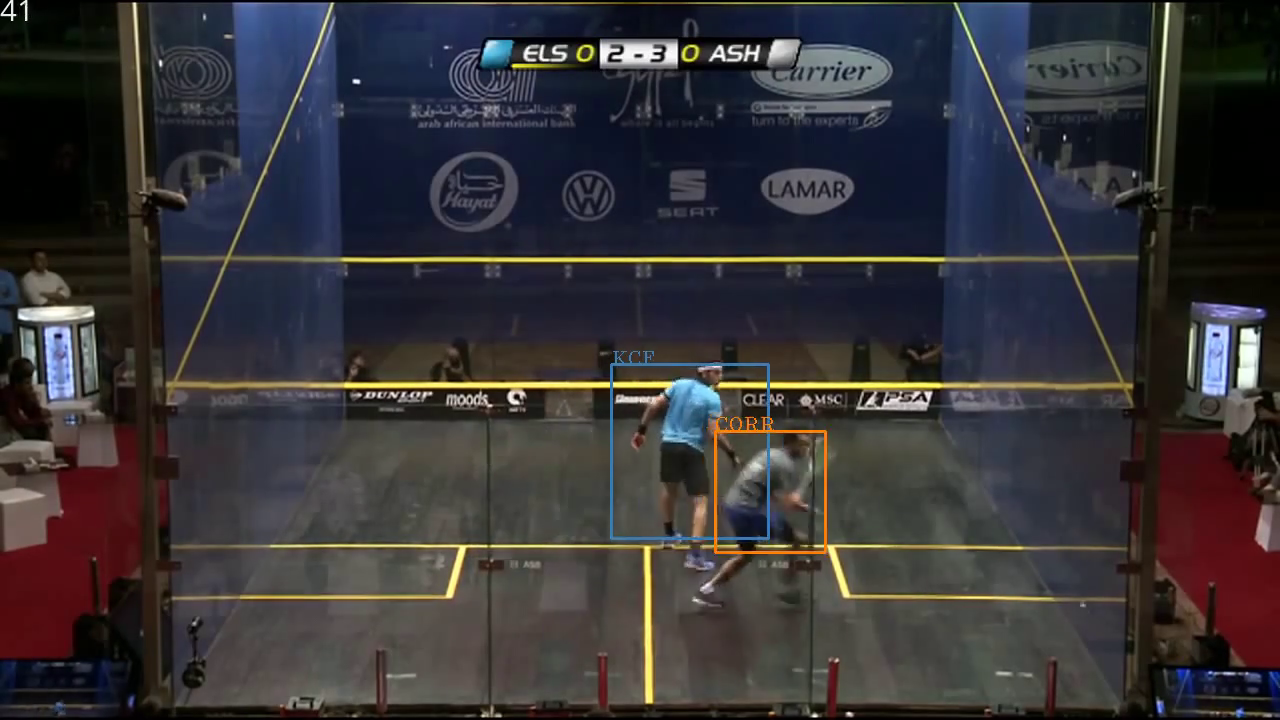
\includegraphics[width=0.6\columnwidth]{preliminary-tracker-squash.png}
	\caption[Primer delovanja sledilnikov za \textit{squash} posnetek]{Primer delovanja sledilnikov za \textit{squash} posnetek. Gre za 41. sliko posnetka \cite{squashtv2014squash}, pri čemer smo uporabili KCF in CORR algoritem. Sledilnika sta morala slediti igralcu z modro majico.}
	\label{fig:squash-tracker-visual}
\end{figure}


Boljše delovanje KCF je razumljivo, saj prvi testi temeljijo na posnetkih rokometa, drugi pa na squashu, kjer gre za bistveno drugačno igro. Če pogledamo tabelo \ref{tab:region-overlap} ima KCF drugo najboljše povprečje, prav tako pa so si rezultati posameznih posnetkov zelo podobni. 


















\subsection{Observabilnost}
Rezultate observabilnosti lahko vidimo v tabeli \ref{tab:observabilnost}. Validacijske metrike so povprečne vrednosti \textit{sv} in \textit{bv} modelov, brez križnega testiranja.  Pearsonov korelacijski koeficient smo povprečili s Fisherjevo $z$ transformacijo. Tako energijska poraba kot srčni utrip, imata visoko pozitivno korelacijo, kar pomeni, da sta oba parametra observabilna. \textit{hr} modeli se po CORR rezultatih bolje ujemajo z referenco, vendar moramo pri tem upoštevati tudi nSV razmerje, ki je tu večje. Če primerjamo metrike napak, \textit{eem} modeli prekašajo \textit{hr} modele. S tem lahko potrdimo, da srčni utrip ni dober fiziološki parameter za določevanje fizične aktivnosti. Najboljši rezultati predikcije energijske porabe in srčnega utripa so prikazani na sliki \ref{fig:stage1-observability}.

\begin{table}[!htbp]
\centering
\begin{tabular}{l S[table-format=1.2, round-mode=places, round-precision=2] S[table-format=1.2, round-mode=places, round-precision=2] S[table-format=1.2, round-mode=places, round-precision=2] S[table-format=1.2, round-mode=places, round-precision=2]}
	\toprule
	\textbf{Model} & \thead{CORR} & \thead{RAE} & \thead{RRSE} & \thead{nSV} \\
		\midrule
		\tdata{observabilnost}
		\bottomrule
		\end{tabular}
		\caption[Validacijske metrike testa observabilnosti]{Validacijske metrike testa observabilnosti. Gre za povprečne vrednosti \textit{sv} in \textit{bv} modelov. Pearsonov korelacijski koeficient (CORR) smo povprečili s Fisherjevo $z$ transformacijo.}
	\label{tab:observabilnost}
	\end{table}
	
\begin{figure}[!htbp]
\centering
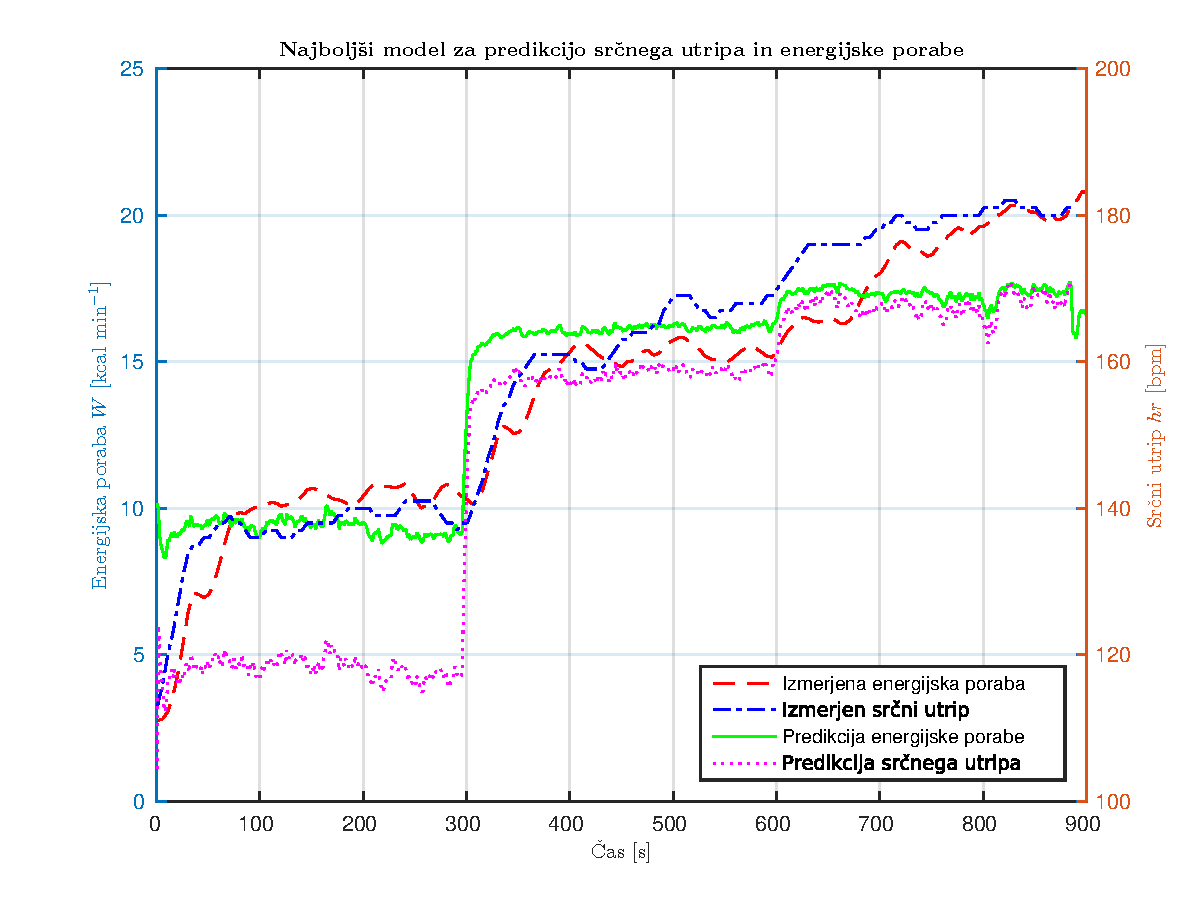
\includegraphics[width=0.5\columnwidth]{best-results-normal--sideview-sideview-normal-sl}
\caption[Najboljši reultati predikcije energijske porabe in srčnega utripa]{Najboljši reultati predikcije energijske porabe in srčnega utripa. Slika prikazuje izhode eem-sv(sv) in hr-sv(sv) modelov ter izmerjene vrednosti energijske porabe in srčnega utripa.}
	\label{fig:stage1-observability}
	\end{figure}


\subsection{Ročni izrez}
Tabela \ref{tab:rocni-izrez} prikazuje rezultate ročnega izreza. Prikazani so tudi rezultati observabilnosti za primerjavo. Validacijske metrike so povprečne vrednosti \textit{sv} in \textit{bv} modelov, brez križnega testiranja.  Pearsonov korelacijski koeficient smo povprečili s Fisherjevo $z$ transformacijo. Rezultati modelov z ročnim izrezovanjem so za malenkost slabši. Še vseeno smo jih uporabili v nadaljnjih testih, ker se z njimi teoretično znebimo šuma ozadja.

\begin{table}[!htbp]
	\centering
	\begin{tabular}{l S[table-format=1.2, round-mode=places, round-precision=2] S[table-format=1.2, round-mode=places, round-precision=2] S[table-format=1.2, round-mode=places, round-precision=2] S[table-format=1.2, round-mode=places, round-precision=2]}
		\toprule
		\textbf{Model} & \thead{CORR} & \thead{RAE} & \thead{RRSE} & \thead{nSV} \\
		\midrule
		\tdata{rocni-izrez}
		\bottomrule
	\end{tabular}
	\caption[Validacijske metrike testov ročnega izreza]{Validacijske metrike testov ročnega izreza. Gre za povprečne vrednosti \textit{sv} in \textit{bv} modelov. Personov korelacijski koeficient (CORR) smo povprečili s Fisherjevo $z$ transformacijo.}
	\label{tab:rocni-izrez}
\end{table}
		
\subsection{Modaliteta}
Rezultati posameznega pogleda kamere so vidni v tabeli \ref{tab:zorni-kot}. Slike smo pred procesiranjem ročno izrezali tako, da smo določili območje tarče, kjer smo zaobjeli celoten subjekt glede na vse sekvence video posnetka. S tem smo simulirali idealni sledilnik. Rezultate tako lažje primerjamo s terenskimi testi.
		
	\begin{table}[!htbp]
	\centering
	\begin{tabular}{l S[table-format=1.2, round-mode=places, round-precision=2] S[table-format=1.2, round-mode=places, round-precision=2] S[table-format=1.2, round-mode=places, round-precision=2] S[table-format=1.2, round-mode=places, round-precision=2]}
\toprule
\textbf{Model} & \thead{CORR} & \thead{RAE} & \thead{RRSE} & \thead{nSV} \\
\midrule
\tdata{zorni-kot}
	\bottomrule
	\end{tabular}
		\caption[Rezultati modalitete zornega kota kamere]{Rezultati modalitete zornega kota kamere.}
		\label{tab:zorni-kot}
		\end{table}
		
Če primerjamo \textit{bv(bv)} in \textit{sv(sv)} modele dobimo pri slednjih boljše rezultate. Slabši rezultati hrbtne kamere bi lahko nakazovali na to, da je ta pogled manj informativen. Pri opazovanju križnih testov (testi s podatki različnega pogleda) lahko vidimo, da dobimo pri vseh slabe rezultate. CORR je zelo nizek ali negativen, metrike napak pa so zelo visoke. Glavna razlika mešanih modelov je opazna šele s primerjavo modelov s križnim testiranjem. Rezultati mešanih modelov so veliko boljši in nakazujejo na to, da lahko dobimo boljše rezultate, če uporabimo podatke iz različnih zornih kotov.

Rezultati različne modalitete glede na tip slike so prikazani v tabeli \ref{tab:zorni-kot}. Tudi tu smo posamezne slike sekvenc posnetkov ročno izrezali. V tabeli je prikazana primerjava \textit{ir} in \textit{bv} modelov. \textit{sv} modelov tu ni, saj smo snemali le hrbtne IR posnetke. Rezultati IR posnetkov so boljši, kar se še posebno opazi pri modelih predikcije srčnega utripa.

\begin{table}[!htbp]
\centering
\begin{tabular}{l S[table-format=1.2, round-mode=places, round-precision=2] S[table-format=1.2, round-mode=places, round-precision=2] S[table-format=1.2, round-mode=places, round-precision=2] S[table-format=1.2, round-mode=places, round-precision=2]}
\toprule
\textbf{Model} & \thead{CORR} & \thead{RAE} & \thead{RRSE} & \thead{nSV} \\
\midrule
\tdata{crop-ir}
	\bottomrule
	\end{tabular}
		\caption[Validacijske metrike glede na tip slike]{Validacijske metrike za različne modalitete glede na tip slike (BGR ali IR).}
		\label{tab:crop-ir}
		\end{table}
	


















\subsection{Modeliranje dodatne zakasnitve}
Modeli z dodatno zakasnitvijo so v tabeli \ref{tab:lag} označeni z \textit{lag}. Opazimo lahko, da so vsi rezultati s zakasnitvijo, ne glede na modaliteto, boljši. Z \textit{lag} modeli smo potrdili predpostavko o zakasnitvi \SI{55}{\s} za energijsko porabo in \SI{15}{\s} za srčni utrip. Ker smo z njimi rešili probleme sinhronizacije, smo jih uporabili v nadaljnjih raziskavah. 

\begin{table}[!htbp]
	\centering
	\begin{tabular}{l S[table-format=1.2, round-mode=places, round-precision=2] S[table-format=1.2, round-mode=places, round-precision=2] S[table-format=1.2, round-mode=places, round-precision=2] S[table-format=1.2, round-mode=places, round-precision=2]}
		\toprule
		\textbf{Model} & \thead{CORR} & \thead{RAE} & \thead{RRSE} & \thead{nSV} \\
		\midrule
		\tdata{crop-lag}
		\bottomrule
	\end{tabular}
	\caption[Primerjava rezultatov med modeli s zakasnitvijo in brez]{Primerjava rezultatov med modeli z dodatno zakasnitvijo in brez.}
	\label{tab:lag}
\end{table}



\begin{figure}[!htbp]
	\centering
	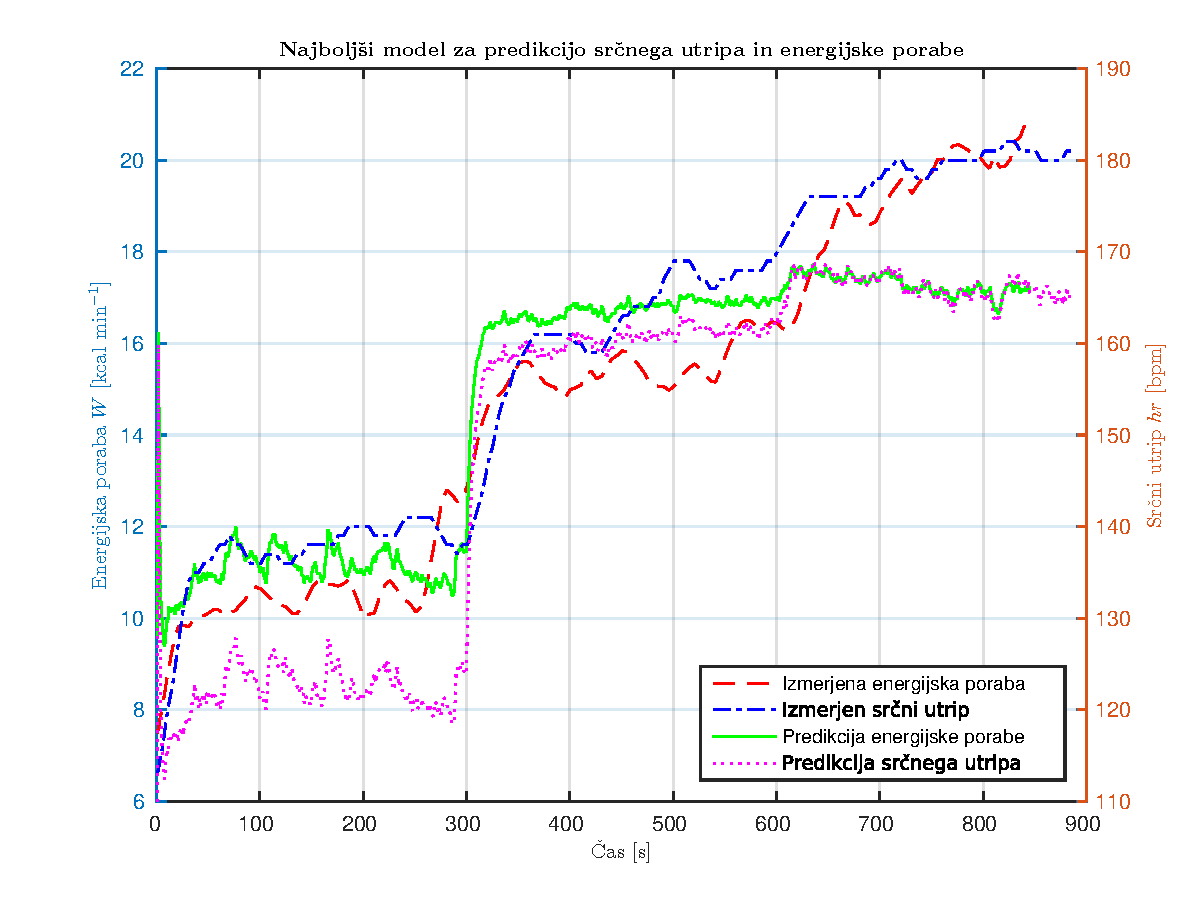
\includegraphics[width=0.5\columnwidth]{best-results-crop-normal-infrared-infrared-lag-sl}
	\caption[Najboljši rezultati predikcije energijske porabe in srčnega utripa s zakasnitvijo]{Najboljši rezultati predikcije energijske porabe in srčnega utripa z upoštevanjem dodatne zakasnitve. Slika prikazuje izhode eem-ir-lag(ir) in hr-ir-lag(ir) modelov ter izmerjene vrednosti energijske porabe in srčnega utripa.}
	\label{fig:crop-lag-rezultat}
\end{figure}

















\subsection{Obremenitveni testi}
Rezultati obremenitvenih testov so prikazani v tabelah \ref{tab:crop-proj} in \ref{tab:crop-scale}. Opazimo lahko, da dobimo pri uporabi IR posnetkov slabše rezultate glede na tabelo \ref{tab:lag}. IR posnetki tako niso primerni za terenske raziskave, saj tam pri snemanju nimamo nikoli idealnih pogojev.

\begin{table}[!htbp]
	\centering
	\begin{tabular}{l S[table-format=1.2, round-mode=places, round-precision=2] S[table-format=1.2, round-mode=places, round-precision=2] S[table-format=1.2, round-mode=places, round-precision=2] S[table-format=1.2, round-mode=places, round-precision=2]}
		\toprule
		\textbf{Model} & \thead{CORR} & \thead{RAE} & \thead{RRSE} & \thead{nSV} \\
		\midrule
		\tdata{crop-proj}
		\bottomrule
	\end{tabular}
	\caption[Validacijske metrike rezultatov s projektivno transformacijo]{Validacijske metrike rezultatov s projektivno transformacijo slik posnetkov.}
	\label{tab:crop-proj}
\end{table}

\begin{table}[!htbp]
	\centering
	\begin{tabular}{l S[table-format=1.2, round-mode=places, round-precision=2] S[table-format=1.2, round-mode=places, round-precision=2] S[table-format=1.2, round-mode=places, round-precision=2] S[table-format=1.2, round-mode=places, round-precision=2]}
		\toprule
		\textbf{Model} & \thead{CORR} & \thead{RAE} & \thead{RRSE} & \thead{nSV} \\
		\midrule
		\tdata{crop-sc}
		\bottomrule
	\end{tabular}
	\caption[Rezultati obremenitvenega testa skaliranja]{Rezultati obremenitvenega testa skaliranja.}
	\label{tab:crop-scale}
\end{table}










\subsection{Tekalna steza s sledenjem}
Pri testiranju vpeljave sledilnika smo dobili rezultate v tabeli \ref{tab:shake}. Z vpeljavo sledilnika smo dobili celo nekoliko boljše rezultate od tistih z ročnim izrezovanjem (tabela \ref{tab:lag}). To si lahko razlagamo s tem, da je z uporabo sledilnika določitev območja tarče bolj optimalno, saj je območje določeno za vsako sliko posebej. Zaradi tega so modeli bolj robustni na šum ozadja.

%Results of models with enabled tracker are represented in Table \ref{tab:tracker-models-validation}. If we compare them with results of initial models in Table \ref{tab:initial-models-validation}, the mean absolute difference of RRSE between them is \SI{28}{\%}. We can assume that this is due to the fact that tracker does not track selected object perfectly. In some cases it cannot find object, or detects wrong object. It can also track only part of the object. This anomalies can affect calculation of physiological parameters.



\begin{table}[!htbp]
	\centering
	\begin{tabular}{l S[table-format=1.2, round-mode=places, round-precision=2] S[table-format=1.2, round-mode=places, round-precision=2] S[table-format=1.2, round-mode=places, round-precision=2] S[table-format=1.2, round-mode=places, round-precision=2]}
		\toprule
		\textbf{Model} & \thead{CORR} & \thead{RAE} & \thead{RRSE} & \thead{nSV} \\
		\midrule
		\tdata{shake}
		\bottomrule
	\end{tabular}
	\caption[Rezultati tekalne steze s sledenjem]{Rezultati tekalne steze s sledenjem. Pri modelih s \textit{sh} kratico smo uporabili simulacijo vibracij. Modeli \textit{tr} so brez vibracij.}
	\label{tab:shake}
\end{table}


Srednja absolutna razlika RRSE metrike med modeli s sledenjem in simulacijo vibracij je okoli \SI{30}{\%}. Rezultati s simulacijo vibracij so slabši, vendar še vedno sprejemljivi, saj sledilnik bolje stabilizira posnetek.











\subsection{Terenski eksperimenti squash igre}
Terenski rezultati squash igre z različnimi deskriptorji so predstavljeni v tabeli \ref{tab:squash}.  Rezultatov ne moremo pravilno evaluirati, ker imamo preobremenjene modele. Zaključimo lahko, da postopek 1. faze ne moremo uporabljati za terenske eksperimente. Odziv preobremenjenih modelov lahko vidimo na sliki \ref{fig:squash-rezultat}.

\begin{table}[!htbp]
	\centering
	\begin{tabular}{l S[table-format=1.2, round-mode=places, round-precision=2] S[table-format=1.2, round-mode=places, round-precision=2] S[table-format=1.2, round-mode=places, round-precision=2] S[table-format=1.2, round-mode=places, round-precision=2]}
		\toprule
		\textbf{Model} & \thead{CORR} & \thead{RAE} & \thead{RRSE} & \thead{nSV} \\
		\midrule
		\tdata{squash-mag}
		\bottomrule
	\end{tabular}
	\caption[Validacijske metrike terenskega testiranja]{Validacijske metrike terenskega testiranja. Tu uporabljamo HOOF in HOOF-HAFA deskriptorje. Modeli so neveljavni.}
	\label{tab:squash}
\end{table}

\begin{figure}[!htbp]
	\centering
	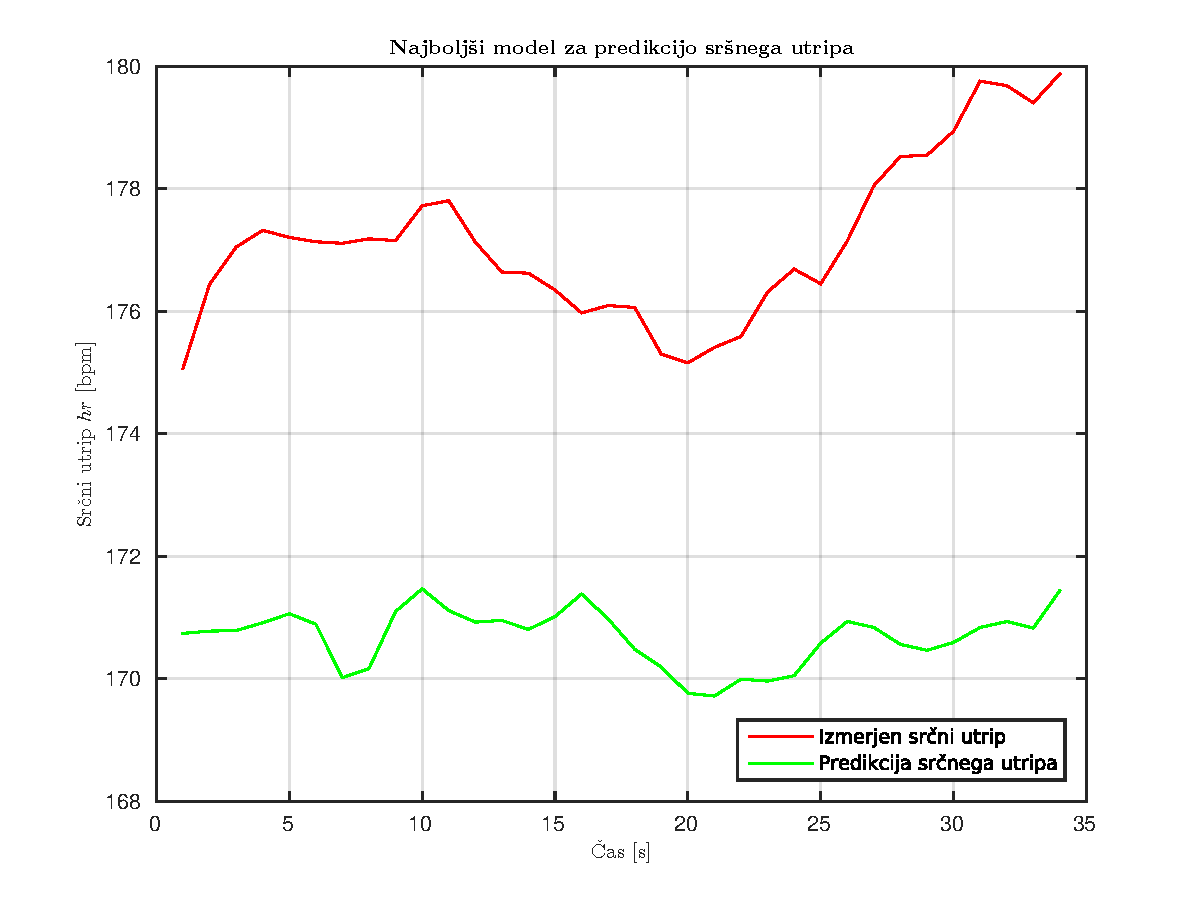
\includegraphics[width=0.5\columnwidth]{best-results-preliminary-squash2-normal-backview-backview-lag-sl}
	\caption[Odziv modela hr-bv-lag-hoofhafa(bv) za terenski eksperiment 1. faze]{Odziv modela hr-bv-lag-hoofhafa(bv) za terenski eksperiment 1. faze.}
	\label{fig:squash-rezultat}
\end{figure}






















\subsection{Eksperiment detekcije dihanja}
Za detekcijo dihanja, ki smo jo formulirali kot problem razvrščanja v razrede, smo uporabili standardne metrike za evaluacijo dvorazrednega problema. ``Diha'' smo označili kot pozitivno vrednost, ``ne diha'' pa negativno. Dobili smo sledeče rezultate: Razmerje napačno potrjenih FPR = \SI{13}{\%}, razmerje pravilno potrjenih TPR = \SI{87}{\%}, razmerje napačno zavrnjenih FNR = \SI{26}{\%}, razmerje pravilno zavrnjenih TNR = \SI{74}{\%}. Rezultati so prav tako prikazani s kontigenčno matriko na sliki \ref{fig:breathtest-confusion} in ROC krivuljno \ref{fig:breathtest-roc}.

\begin{figure}[!htbp]
	\centering
	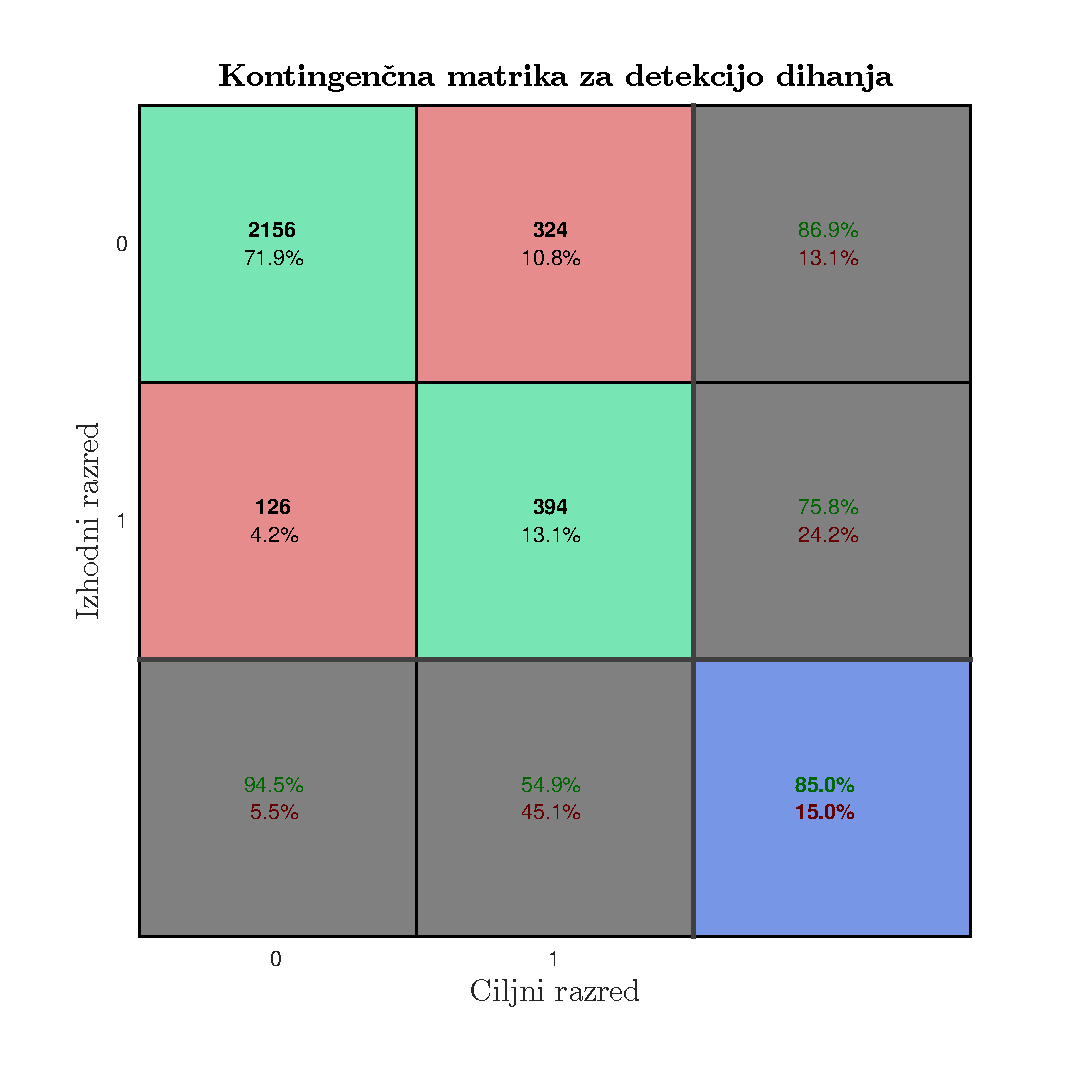
\includegraphics[width=0.5\linewidth]{breathtest-confusion-sl}
	\caption[Kontigenčna matrika za detekcijo dihanja]{Kontigenčna matrika med ciljnim in izhodnim razredom za detekcijo dihanja. Razred $1$ pomeni ``diha''. Razred $0$ pomeni ``ne diha''.}
	\label{fig:breathtest-confusion}
\end{figure}

\begin{figure}[!htbp]
	\centering
	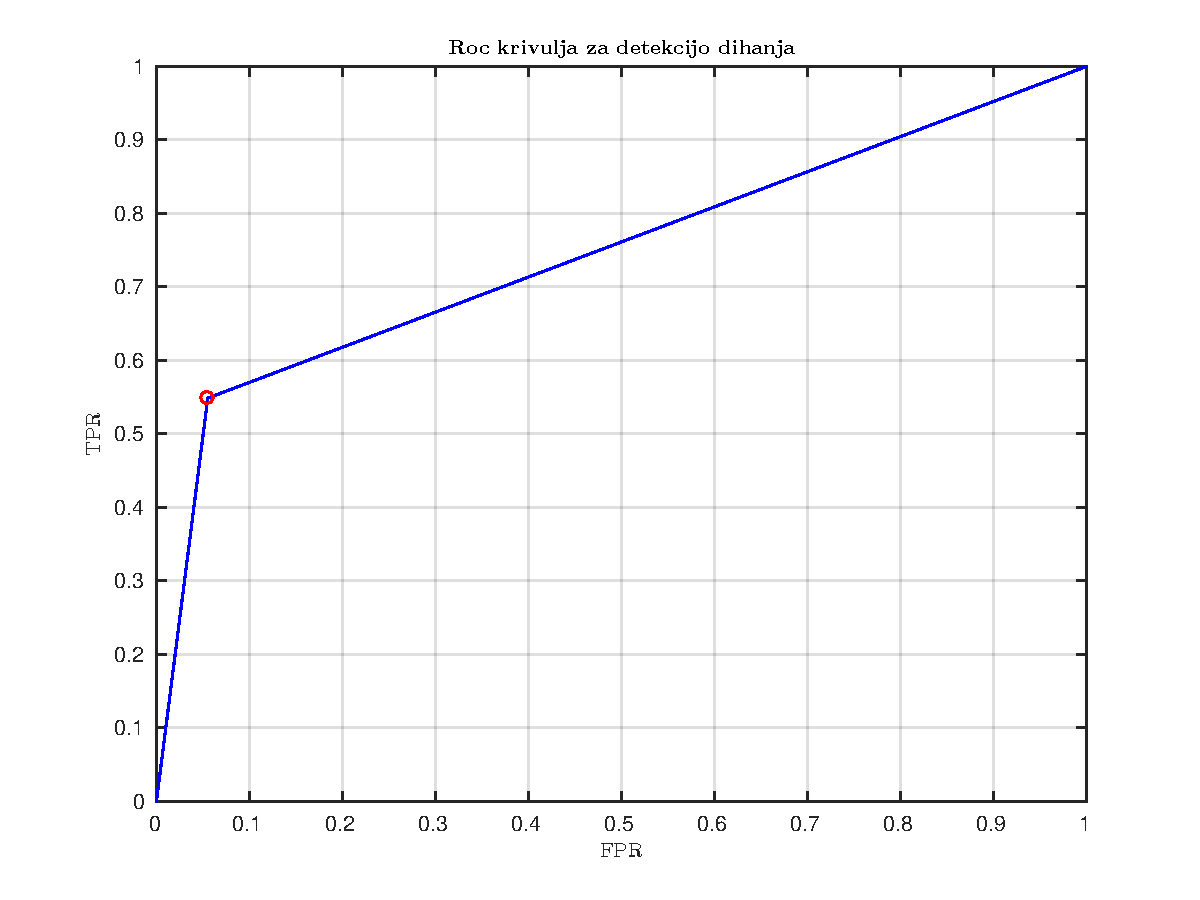
\includegraphics[width=0.5\linewidth]{breathtest-roc-sl}
	\caption[ROC krivulja za detekcijo dihanja]{ROC krivulja za detekcijo dihanja.}
	\label{fig:breathtest-roc}
\end{figure}




























\section{Eksperimenti 2. faze}
\subsection{Preliminarni eksperimenti}
\subsubsection{Združevanje slik iz dveh Kinect kamer}\label{sec:rezultati-zdruzevanje}
Združevanje s značilkami se ni obneslo, zato smo to metodo opustili. Primer neuspelega poskusa je prikazan na sliki \ref{fig:zdruzevanje-znacilke}.

\begin{figure}[!htb]
	\centering
	\begin{subfigure}[t]{0.45\columnwidth}
		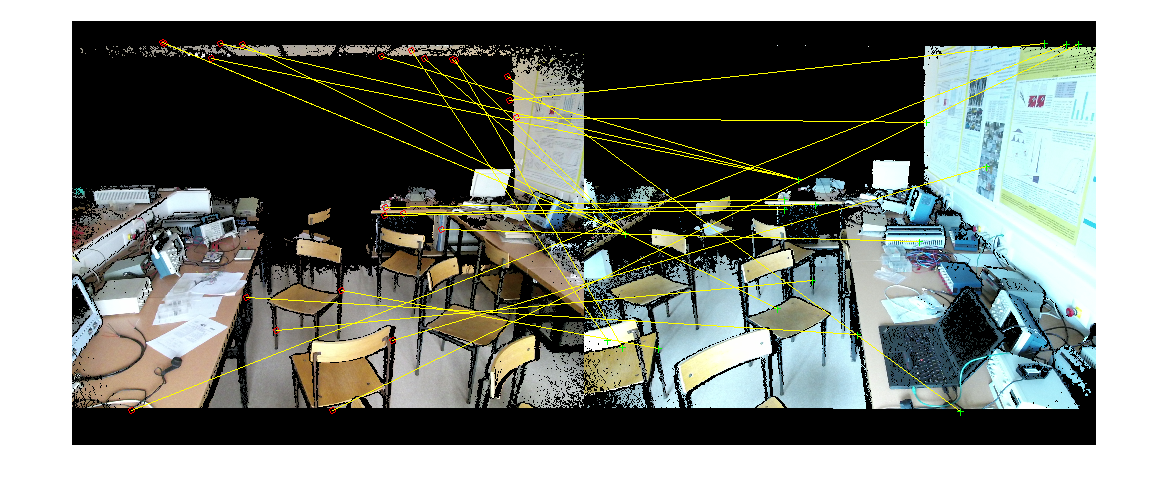
\includegraphics[width=\columnwidth]{./Slike/matched-features.png}
		\caption{Ujemajoče SURF značilke}
		\label{fig:zdruzevanje-surf}
	\end{subfigure}
	~
	\begin{subfigure}[t]{0.45\columnwidth}
		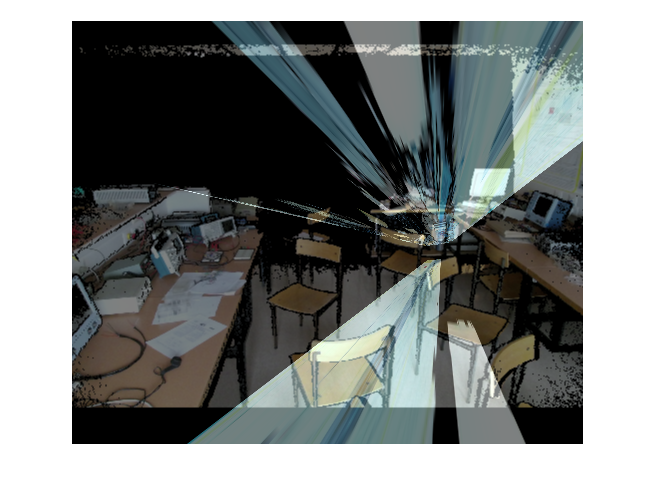
\includegraphics[width=\columnwidth]{./Slike/features-calibration-result.png}
		\caption{Rezultat združevanja z značilkami}
		\label{fig:zdruzevanje-result}
	\end{subfigure}
	\caption[Neuspelo združevanje slik s SURF značilkami]{Primer neuspelega poskusa združevanja slik iz dveh Kinect kamer s SURF značilkami.}
	\label{fig:zdruzevanje-znacilke}
\end{figure}

 Rezultat združevanja s kontrolnimi točkami je bil boljši od združevanja z značilkami, vendar še vedno slab, zato smo tudi to metodo opustili. Primer neuspelega poskusa je prikazan na sliki \ref{fig:zdruzevanje-cp}.
 
 \begin{figure}[!htb]
 	\centering
 	\begin{subfigure}[t]{0.45\columnwidth}
 		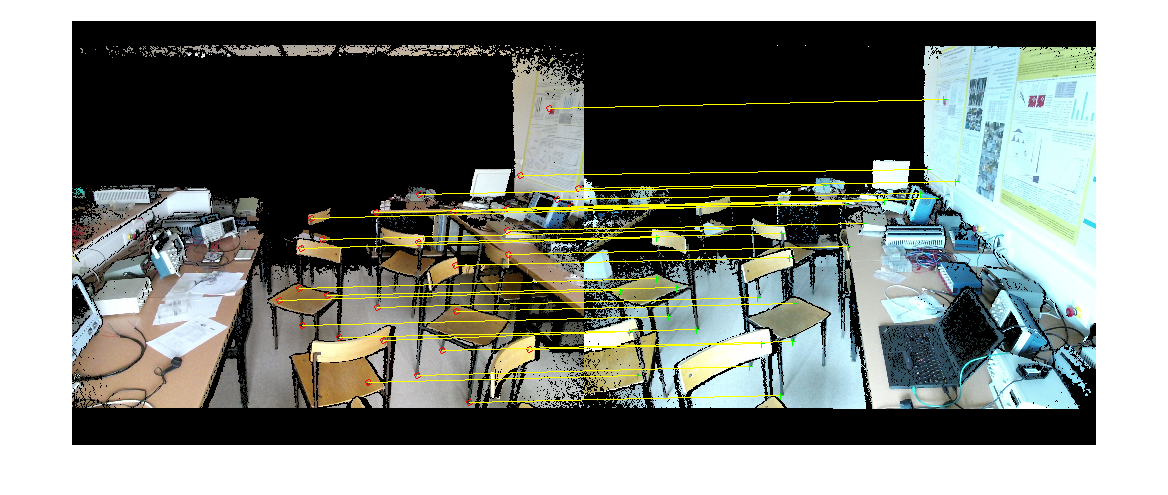
\includegraphics[width=\columnwidth]{matched-points.png}
 		\caption{Ujemajoče kontrolne točke}
 		\label{fig:zdruzevanje-ujemajoce-cp}
 	\end{subfigure}
 	~
 	\begin{subfigure}[t]{0.45\columnwidth}
 		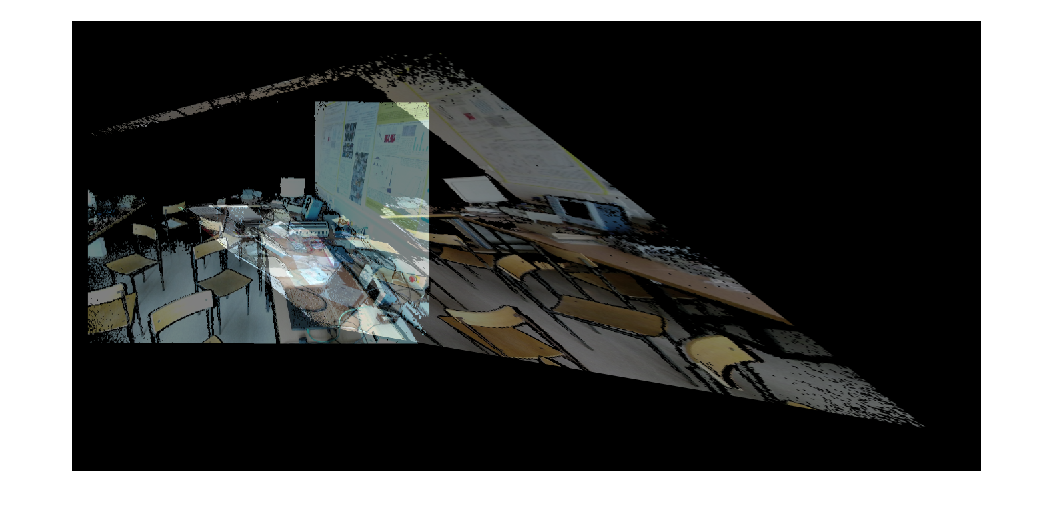
\includegraphics[width=\columnwidth]{points-calibration-result.png}
 		\caption{Rezultat združevanja s kontrolnimi točkami}
 		\label{fig:zdruzevanje-result-cp}
 	\end{subfigure}
 	\caption[Neuspelo združevanje slik s kontrolnimi točkami]{Primer neuspelega poskusa združevanja slik iz dveh Kinect kamer s kontolnimi točkami.}
 	\label{fig:zdruzevanje-cp}
 \end{figure}











\subsubsection{Optimizacija Gaussovega filtra}
Rezultati povprečnih vrednosti uporabljenih metrik so vidni v tabeli \ref{tab:gauss}. Za pravilno razlago rezultatov, moramo upoštevati tudi grafe metrik posameznih eksperimentov, ki so prikazani na slikah \ref{fig:sigma1-5}, \ref{fig:sigma-rmse5-21} in \ref{fig:sigma21-51}. 



\begin{table}[!htb]
	\centering
	\begin{tabular}{S[table-format=2.0, round-mode=places, round-precision=2] S[table-format=1.2, round-mode=places, round-precision=2] S[table-format=2.2, round-mode=places, round-precision=2]}
		\toprule
		\thead{$\mathbf{\sigma}$} & \thead{RMSE} & \thead{SNR [dB]}  \\
		\midrule
		1 & 4.7764 & 24.1892\\
		3 & 6.3162 & 25.5183\\
		5 & 6.5385 & 25.8459\\
		11 & 6.6457 & 26.1244\\
		21 & 6.6794 & 26.2933\\
		31 & 6.6951 & 26.3922\\
		51 & 6.7155 & 26.5345\\
		\bottomrule
	\end{tabular}
	\caption[Metrike pri optimizaciji Gaussovega filtra]{Povprečne vrednosti RMSE in SNR metrik pri optimizaciji parametra $\sigma$ Gaussovega filtra. Najmanjši standardni odklon ima najmanjšo napako, vendar je tudi filtriranje majhno. Pri $\sigma=3$ in $\sigma=5$ so še opazne razlike pri filtriranju. Za višje vrednosti ni več opazne razlike, vendar pa se napaka povečuje. $\sigma=5$ je tako optimalna vrednosti parametra.}
	\label{tab:gauss}
\end{table}

Najmanjšo napako dobimo, če uporabimo $\sigma=1$, vendar pa imamo pri tem najmanjše filtriranje, zato so rezultati še vedno lahko zelo šumni. Z višanjem parametra filtra, se napaka po metriki RMSE povečuje, vendar ima večji vpliv razmerje SNR, saj je predstavljeno v logaritemski skali. 

\begin{figure}[!htb]
	\centering
	\begin{subfigure}[t]{0.45\columnwidth}
		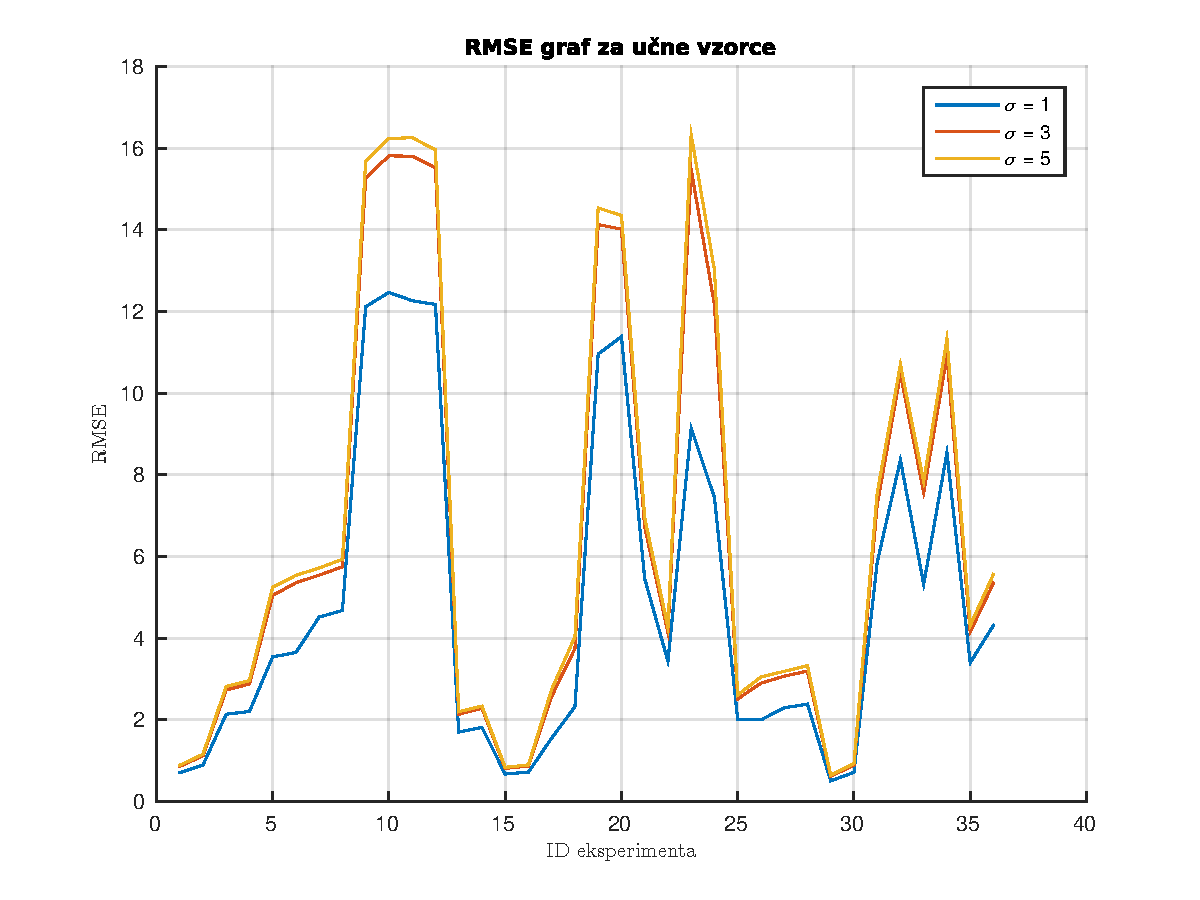
\includegraphics[width=\columnwidth]{sigma-rmse1-5-sl}
		\caption{Graf RMSE  učnih vzorcev }
		\label{fig:sigma-rmse1-5}
	\end{subfigure}
	~
	\begin{subfigure}[t]{0.45\columnwidth}
		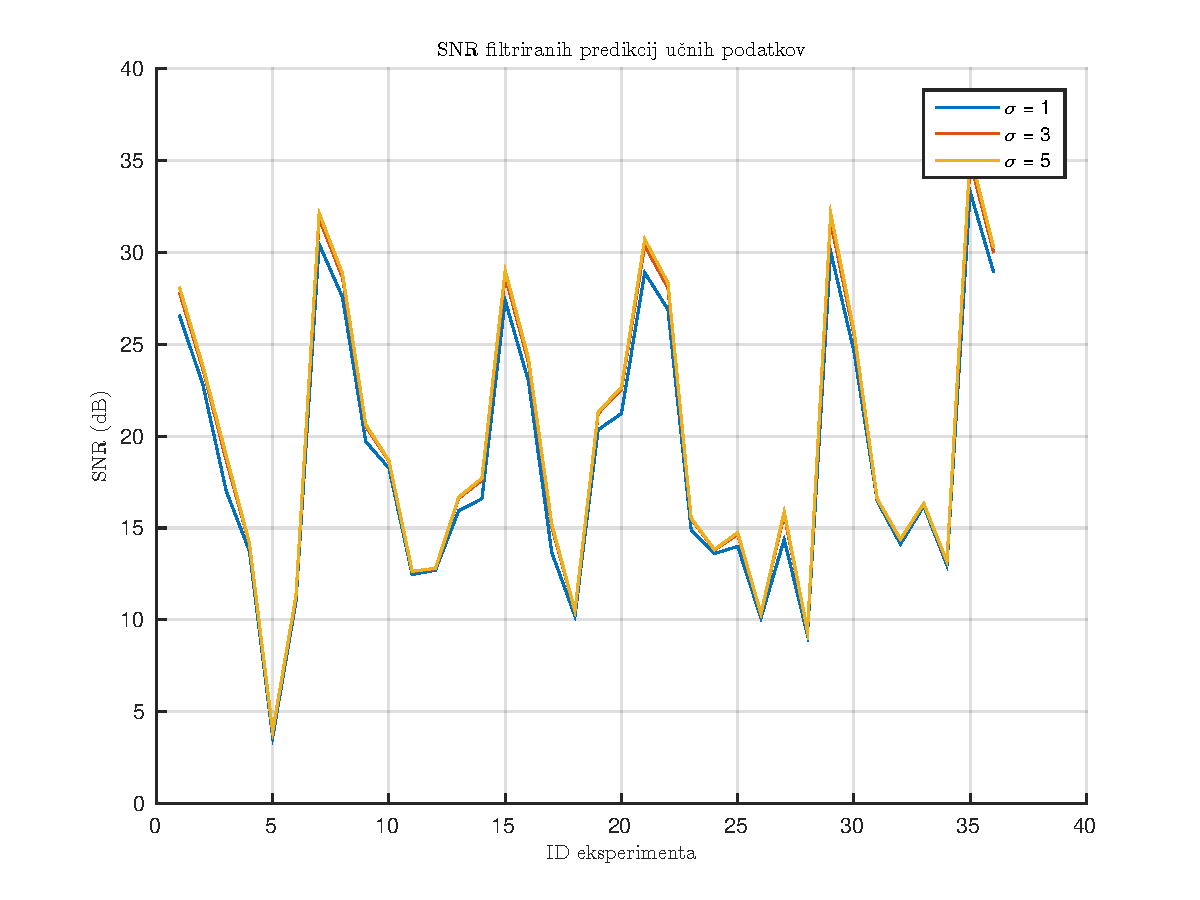
\includegraphics[width=\columnwidth]{sigma-snr1-5-sl}
		\caption{Graf SNR  učnih vzorcev}
		\label{fig:sigma-snr1-5}
	\end{subfigure}
	\caption{Grafa RMSE in SNR učnih vzorcev za \mbox{$\sigma \in [1,5]$}}
	\label{fig:sigma1-5}
\end{figure}

Čeprav pri uporabi $\sigma=51$ dobimo največje filtriranje šuma, lahko na slikah grafov opazimo, da se obe metriki bistveno ne razlikujeta za vrednosti parametra na intervalu $[5,51]$. Kljub dobremu filtriranju želimo zagotoviti čim manjšo napako med referenčnim signalom in predikcijo, zato je logična izbira čim manjši standardni odklon. Ker so na sliki \ref{fig:sigma1-5} med $\sigma=3$ in $\sigma=5$ še opazne razlike, lahko zaključimo, da je $\sigma=5$ optimalna izbira parametra za naš problem. 


\begin{figure}[!htb]
	\centering
	\begin{subfigure}[t]{0.45\columnwidth}
		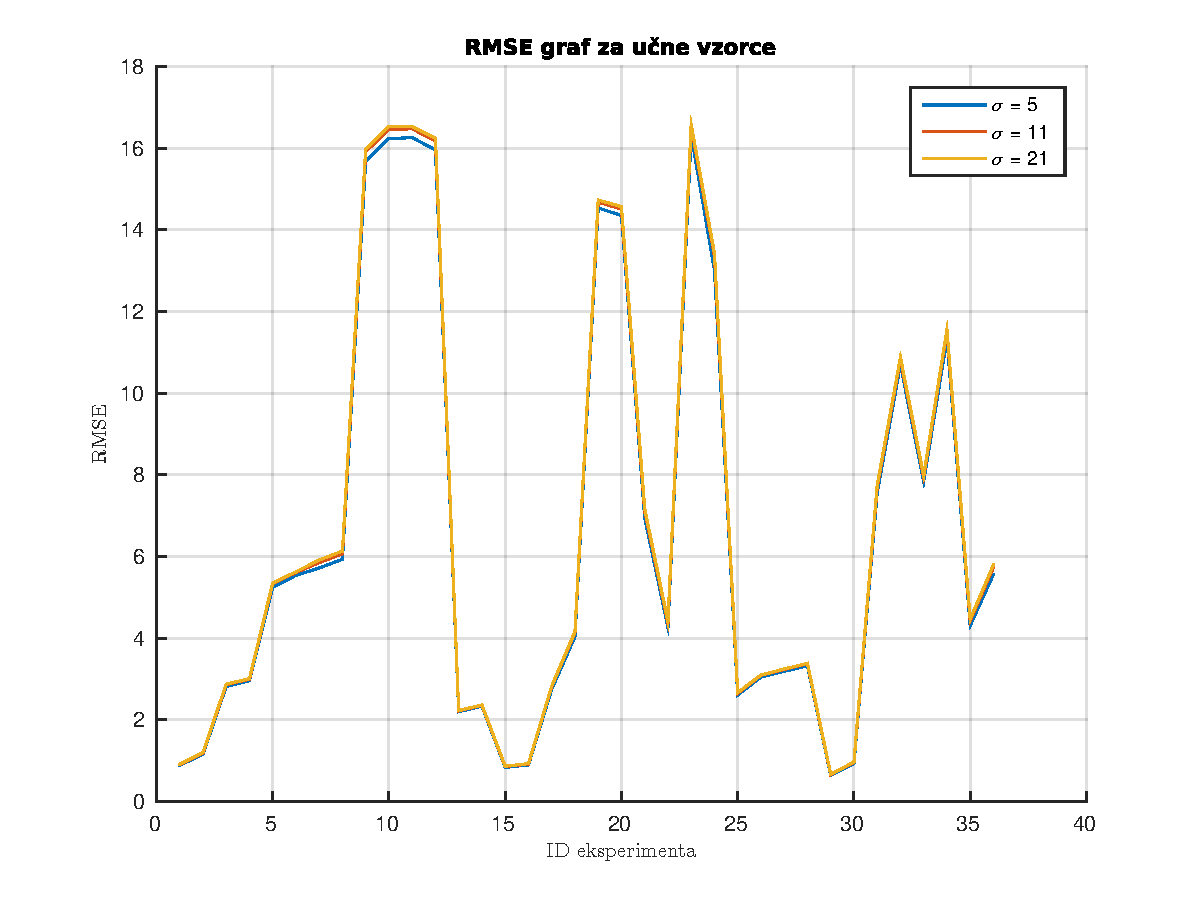
\includegraphics[width=\columnwidth]{sigma-rmse5-21-sl}
		\caption{Graf RMSE  učnih vzorcev}
		\label{fig:sigma-rmse5-21}
	\end{subfigure}
	~
	\begin{subfigure}[t]{0.45\columnwidth}
		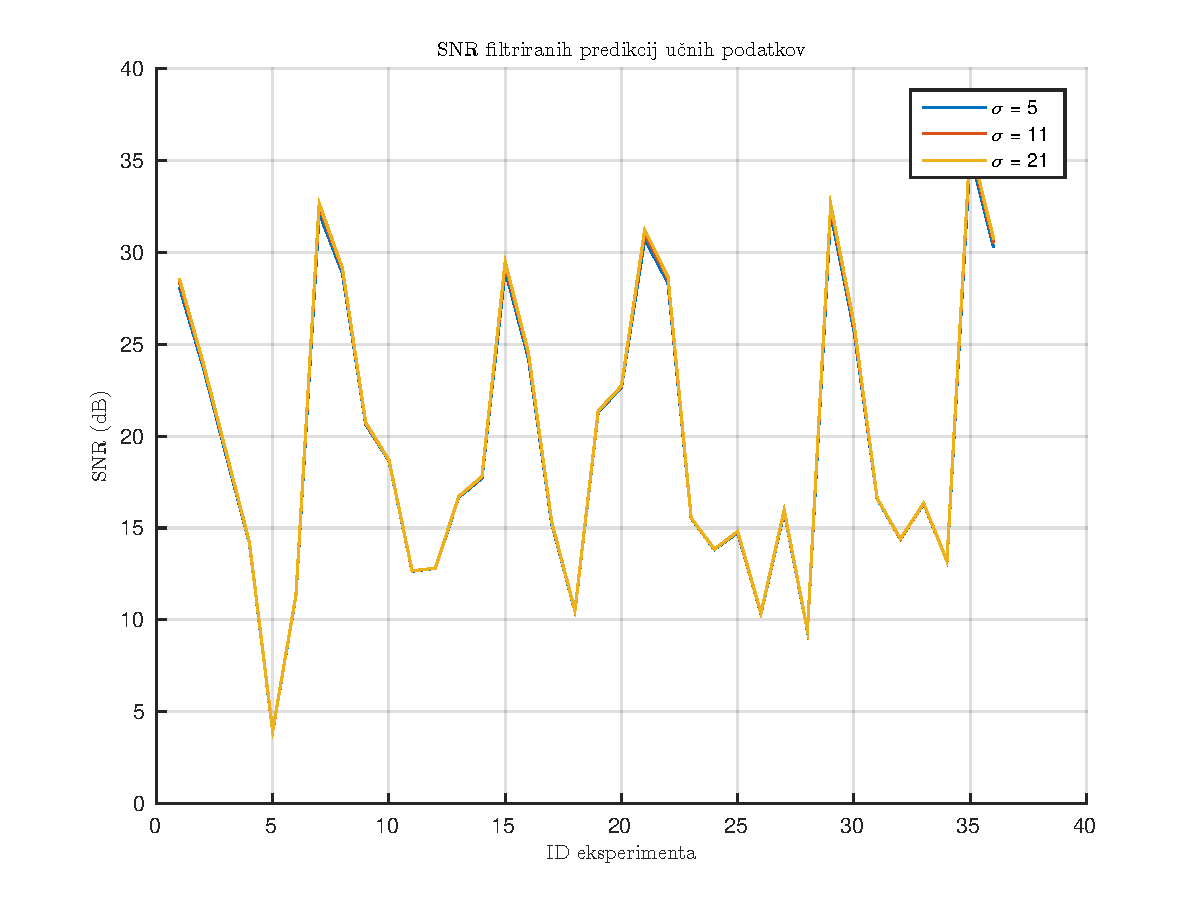
\includegraphics[width=\columnwidth]{sigma-snr5-21-sl}
		\caption{Graf SNR  učnih vzorcev}
		\label{fig:sigma-snr5-21}
	\end{subfigure}
	\caption[Grafa RMSE in SNR učnih vzorcev za \mbox{$\sigma \in [5,21]$}]{Grafa RMSE in SNR učnih vzorcev za \mbox{$\sigma \in [5,21]$}.}
	\label{fig:sigma5-21}
\end{figure}



\begin{figure}[!htb]
	\centering
	\begin{subfigure}[t]{0.45\columnwidth}
		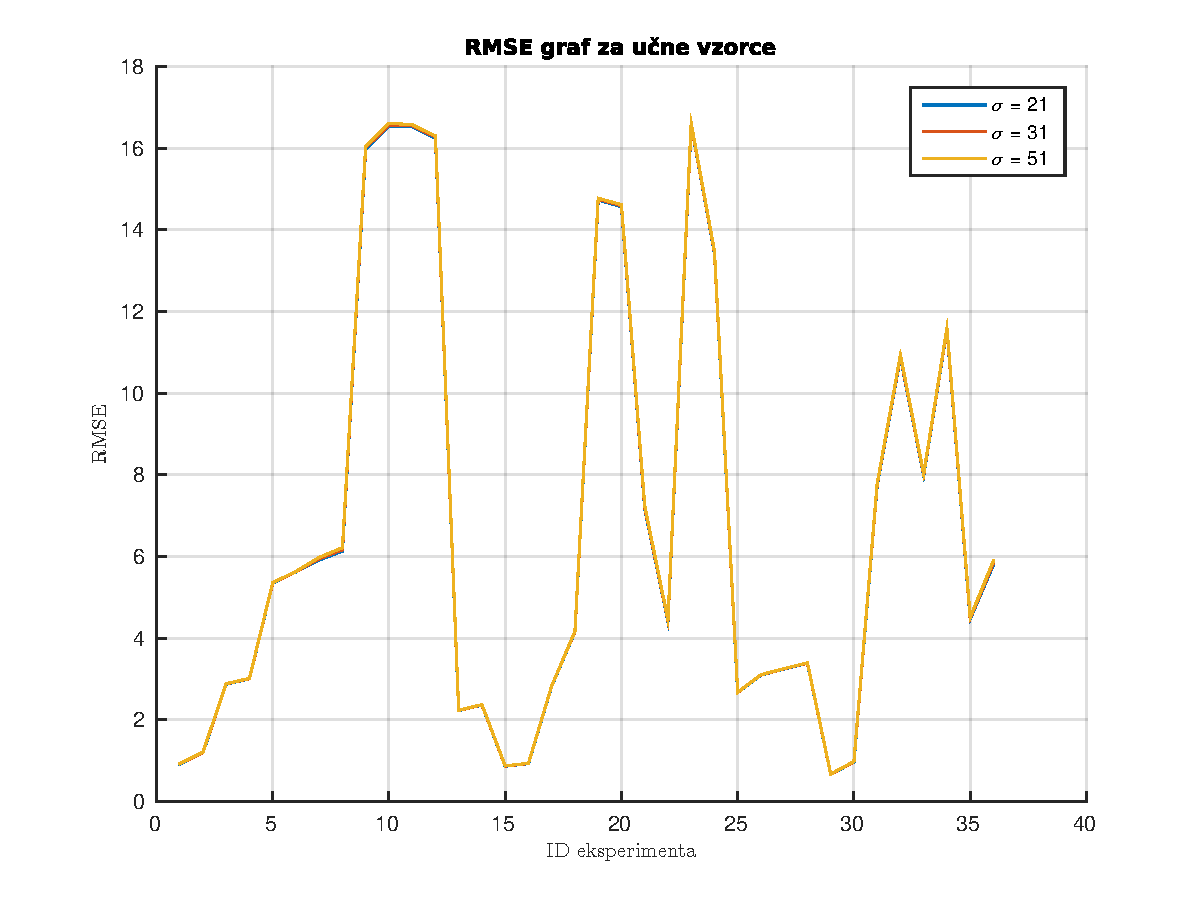
\includegraphics[width=\columnwidth]{sigma-rmse21-51-sl}
		\caption{Graf RMSE učnih vzorcev}
		\label{fig:sigma-rmse21-51}
	\end{subfigure}
	~
	\begin{subfigure}[t]{0.45\columnwidth}
		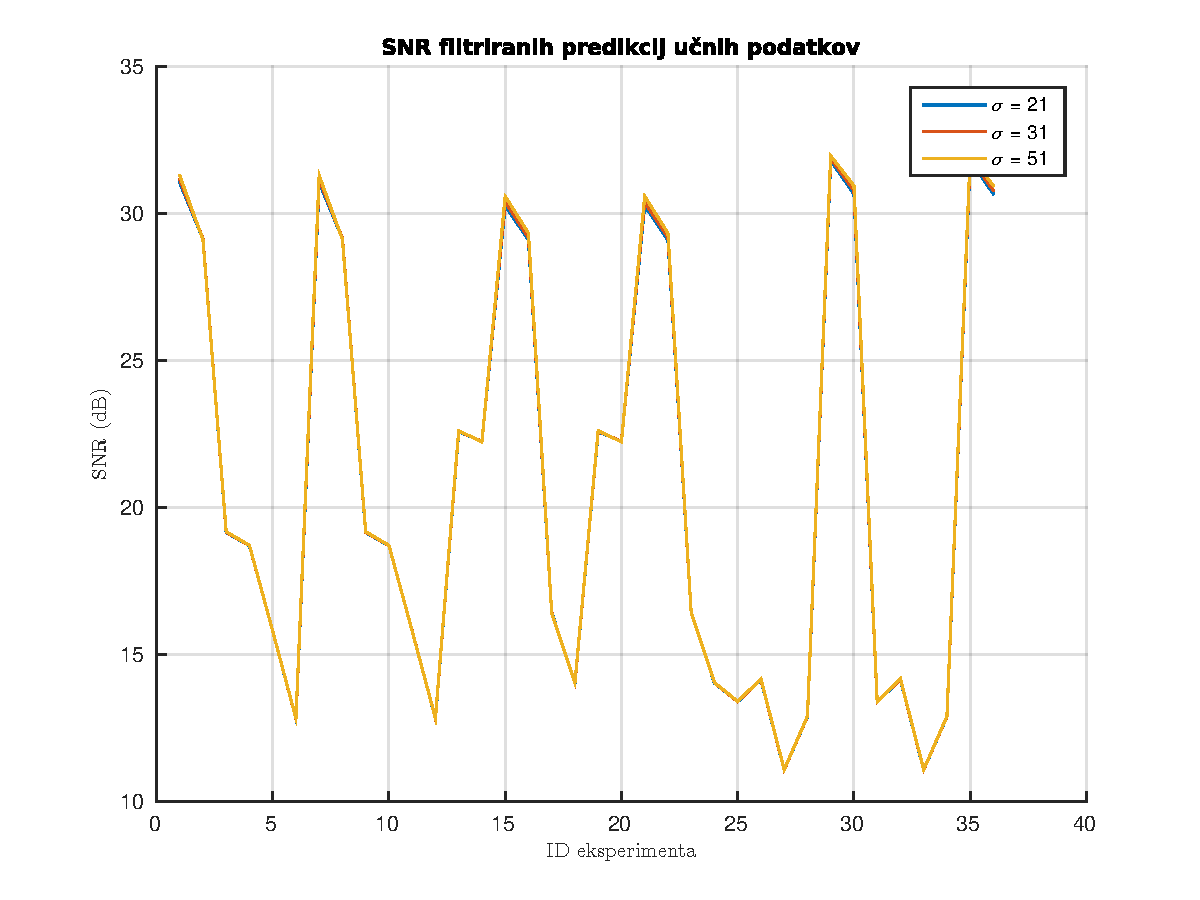
\includegraphics[width=\columnwidth]{sigma-snr21-51-sl}
		\caption{Graf SNR  učnih vzorcev}
		\label{fig:sigma-snr21-51}
	\end{subfigure}
	\caption[Grafa RMSE in SNR učnih vzorcev za \mbox{$\sigma \in [21,51]$}]{Grafa RMSE in SNR učnih vzorcev za \mbox{$\sigma \in [21,51]$}.}
	\label{fig:sigma21-51}
\end{figure}


\subsubsection{Rezultati mrežnega iskanja \texorpdfstring{$\nu$}{nu}-RBF}
Rezultati optimizacije parametra $\numax$ so predstavljeni v tabeli \ref{tab:nu-max}. Pri validaciji ni opaznih sprememb med različnim parametrom $\numax$ zaradi slabih modelov, zato smo preverili verifikacijo. Pri verifikaciji lahko opazimo, da se s povečevanjem parametra povečuje število podpornih vektorjev, vendar nSV nikoli ne doseže željene vrednosti $\numax$. Kljub podoptimalnosti modelov, z višjimi vrednostmi $\numax$ dobimo boljše rezultate. Razlike med $\numax=0.5$ in $\numax=0.8$ so minimalne zato lahko zaključimo, da potrebujemo za dobro delovanje vsaj $\numax=0.5$. 

\begin{table}[!htbp]
	\centering
	\begin{tabular}{l S[table-format=1.2, round-mode=places, round-precision=2] S[table-format=1.2, round-mode=places, round-precision=2] S[table-format=1.2, round-mode=places, round-precision=2] S[table-format=1.2, round-mode=places, round-precision=2]}
		\toprule
		\textbf{Model} & \thead{CORR} & \thead{RAE} & \thead{RRSE} & \thead{nSV} \\
		\midrule
		\tdata{nu-max}
		\bottomrule
	\end{tabular}
	\caption[Verifikacijske metrike pri optimizaciji parametra $\numax$]{Verifikacijske metrike pri optimizaciji parametra $\numax$ postopka mrežnega iskanja \nurbf.}
	\label{tab:nu-max}
\end{table}


Tabela \ref{tab:rbf-nu} predstavlja primerjavo med postopkom z uporabo \nurbf in brez. Metrike so povprečne vrednosti \textit{sv} in \textit{bv} modalitet, pri čemer nismo upoštevali ročnega izrezovanja slik. Pearsonov korelacijski koeficient (CORR) smo povprečili s Fisherjevo $z$ transformacijo. Rezultati nakazujejo, da lahko z uporabo \nurbf dobimo izboljšane rezultate.

\begin{table}[!htbp]
	\centering
	\begin{tabular}{l S[table-format=1.2, round-mode=places, round-precision=2] S[table-format=1.2, round-mode=places, round-precision=2] S[table-format=1.2, round-mode=places, round-precision=2] S[table-format=1.2, round-mode=places, round-precision=2]}
		\toprule
		\textbf{Model} & \thead{CORR} & \thead{RAE} & \thead{RRSE} & \thead{nSV} \\
		\midrule
		\tdata{rbf-nu}
		\bottomrule
	\end{tabular}
	\caption[Validacijske metrike za primerjavo med \nurbf in klasičnim modelom]{Validacijske metrike za primerjavlo med postopkom z \nurbf in brez. Gre za povprečne vrednosti \textit{sv} in \textit{bv} modelov. Pearsonov korelacijski koeficient (CORR) smo povprečili s Fisherjevo $z$ transformacijo.}
	\label{tab:rbf-nu}
\end{table}




\begin{comment}
\subsubsection{Jedro GHI}
\begin{table}[!htbp]
	\centering
	\begin{tabular}{l S[table-format=1.2, round-mode=places, round-precision=2] S[table-format=1.2, round-mode=places, round-precision=2] S[table-format=1.2, round-mode=places, round-precision=2] S[table-format=1.2, round-mode=places, round-precision=2]}
		\toprule
		\textbf{Model} & \thead{CORR} & \thead{RAE} & \thead{RRSE} & \thead{nSV} \\
		\midrule
		\bottomrule
	\end{tabular}
	\caption{Ghi vmax800}
	\label{tab:ghi}
\end{table}

\begin{figure}[!htbp]
	\centering
	\caption{Ghi best - eem-sv-lag(sv)}
	\label{fig:ghi}
\end{figure}
\end{comment}


\subsubsection{Normalizacija HAFA deskriptorja}
V tabeli \ref{tab:norm-hafa} dobimo slabe rezultate tako za NORMAL model kot tudi za DIAG model, kjer upoštevamo amplitudni faktor $f_A$. Kljub temu so rezultati z upoštevanjem diagonale boljši, kar nakazuje tudi slika \ref{fig:corr-diag}.

\begin{table}[!htbp]
	\centering
	\begin{tabular}{l S[table-format=1.2, round-mode=places, round-precision=2] S[table-format=1.2, round-mode=places, round-precision=2] S[table-format=1.2, round-mode=places, round-precision=2] S[table-format=1.2, round-mode=places, round-precision=2]}
		\toprule
		\textbf{Model} & \thead{CORR} & \thead{RAE} & \thead{RRSE} & \thead{nSV} \\
		\midrule
		\tdata{diag}
		\bottomrule
	\end{tabular}
	\caption[Evaluacijske metrike pri primerjavi modelov NORMAL in DIAG]{Evaluacijske metrike pri primerjavi modelov NORMAL in DIAG, kjer upoštevamo amplitudni faktor $f_A$. }
	\label{tab:norm-hafa}
\end{table}

\begin{figure}[!htb]
	\centering
	\begin{subfigure}[t]{0.45\columnwidth}
		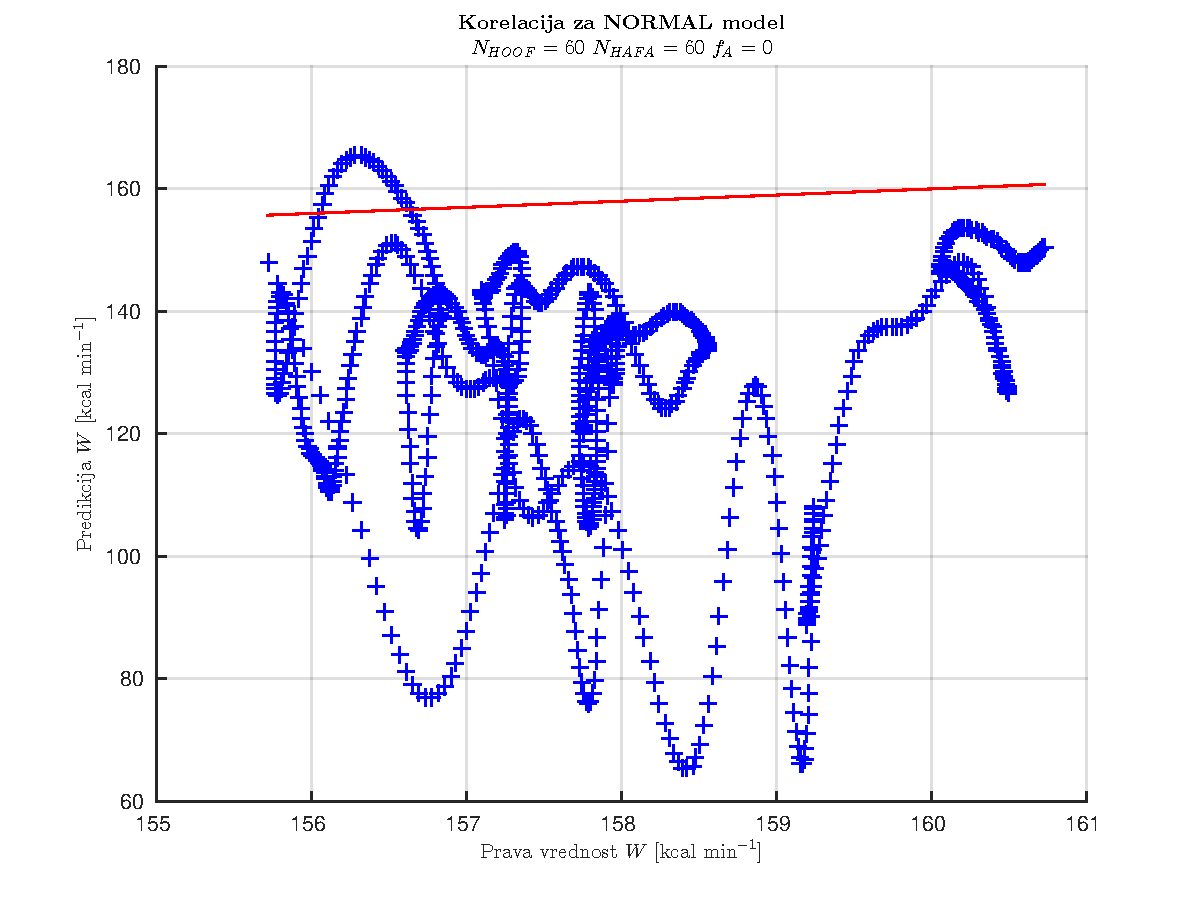
\includegraphics[width=\columnwidth]{diag-normal-corr-sl}
		\caption{Korelacija za NORMAL model.}
		\label{fig:corr-diag-normal}
	\end{subfigure}
	~
	\begin{subfigure}[t]{0.45\columnwidth}
		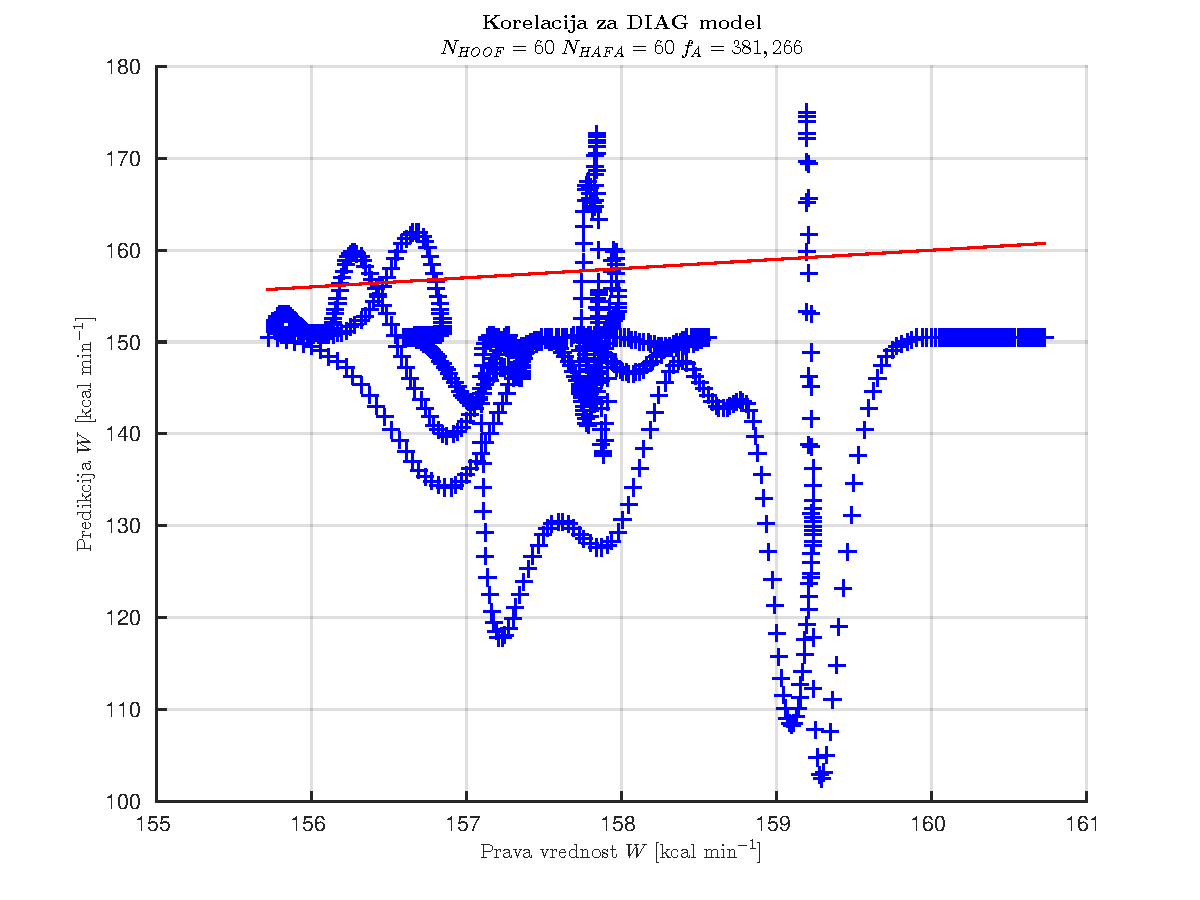
\includegraphics[width=\columnwidth]{diag-diag-corr-sl}
		\caption{Korelacija za DIAG model.}
		\label{fig:corr-diag-diag}
	\end{subfigure}
	\caption[]{Grafa korelacij za NORMAL in DIAG model. Kljub slabim rezultatom obeh modelov, je DIAG model občutno boljši.}
	\label{fig:corr-diag}
\end{figure}


\subsection{Laboratorijski eksperiementi}
\subsubsection{Odvisnost na akumulacijo utrujenosti}
V tabeli \ref{tab:stage2-lab-1-mean} je predstavljeno povprečje validacij merjencev za protokol 1. Pearsonov korelacijski koeficient (CORR) smo povprečili s Fisherjevo $z$ transformacijo. Vsi modeli imajo visoko korelacijo z referenco. Napake so majhne. Opazimo, da dobimo boljše rezultate z uporabo prostorskega toka \textit{it}.

\begin{table}[!htbp]
	\centering
	\begin{tabular}{l S[table-format=1.2, round-mode=places, round-precision=2] S[table-format=1.2, round-mode=places, round-precision=2] S[table-format=1.2, round-mode=places, round-precision=2] S[table-format=1.2, round-mode=places, round-precision=2]}
		\toprule
		\textbf{Model} & \thead{CORR} & \thead{RAE} & \thead{RRSE} & \thead{nSV} \\
		\midrule
		\tdata{stage2-lab-1-mean}
		\bottomrule
	\end{tabular}
	\caption[Povprečje validacij merjencev za protokol 1 2. faze lab. eksperimentov]{Povprečje validacij merjencev za protokol 1 druge faze laboratorijskih eksperimentov. Personov korelacijski koeficient (CORR) smo povprečili s Fisherjevo $z$ transformacijo.}
	\label{tab:stage2-lab-1-mean}
\end{table}

V tabeli \ref{tab:stage2-lab-2-mean}  predstavljamo povprečje rezultatov za protokol 2. Pearsonov korelacijski koeficient (CORR) smo povprečili s Fisherjevo $z$ transformacijo. Vsi modeli imajo pričakovano nizko korelacijo in veliko napak.

\begin{table}[!htbp]
	\centering
	\begin{tabular}{l S[table-format=1.2, round-mode=places, round-precision=2] S[table-format=1.2, round-mode=places, round-precision=2] S[table-format=1.2, round-mode=places, round-precision=2] S[table-format=1.2, round-mode=places, round-precision=2]}
		\toprule
		\textbf{Model} & \thead{CORR} & \thead{RAE} & \thead{RRSE} & \thead{nSV} \\
		\midrule
		\tdata{stage2-lab-2-mean}
		\bottomrule
	\end{tabular}
	\caption[Povprečje validacij merjencev za protokol 2 2. faze lab. eksperimentov]{Povprečje validacij merjencev za protokol 2 druge faze laboratorijskih eksperimentov. Pearsonov korelacijski koeficient (CORR) smo povprečili s Fisherjevo $z$ transformacijo.}
	\label{tab:stage2-lab-2-mean}
\end{table}

Glede na rezultate v tabelah \ref{tab:stage2-lab-1-mean} in  \ref{tab:stage2-lab-2-mean} se utrujenost akumulira skozi čas, kar moramo upoštevati pri gradnji modelov.


\subsubsection{Generalizacija modela}
S protokolom 3 smo želeli preveriti, če lahko uporabimo generaliziran model za predikcijo energijske porabe na različnih merjencih. Rezultati so vidni v tabeli \ref{tab:stage2-lab-3}. Zanimivo dobimo najboljše rezultate za optični tok in ne za prostorskega, kot smo predlagali. Korelacije modelov z optičnim tokom \textit{of} se bližajo vrednosti $1$, vendar pa so metrike napak slabše. Nakazujejo na to, da modeli le niso tako zelo dobri. Vsekakor imamo podobne rezultate tako za SUBJ8 kot za SUBJ9, kar naznanja dobro generalizacijo modela.

\begin{table}[!htbp]
	\centering
	\begin{tabular}{l S[table-format=1.2, round-mode=places, round-precision=2] S[table-format=1.2, round-mode=places, round-precision=2] S[table-format=1.2, round-mode=places, round-precision=2] S[table-format=1.2, round-mode=places, round-precision=2]}
		\toprule
		\textbf{Model} & \thead{CORR} & \thead{RAE} & \thead{RRSE} & \thead{nSV} \\
		\midrule
		\tdata{stage2-lab-3}
		\bottomrule
	\end{tabular}
	\caption[Validacijske metrike za protokol 3 2. faze lab. eksperimentov]{Validacijske metrike za protokol 3 druge faze laboratorijskih eksperimentov.}
	\label{tab:stage2-lab-3}
\end{table}

Najboljši rezultati za optični in prostorski tok, so predstavljeni na sliki \ref{fig:lab-3}. Odzivi modelov vsebujejo veliko šuma, zato bi lahko uporabili širše Gaussovo jedro za filtriranje rezultatov. Najslabšo predikcijo dobimo za največjo fizično aktivnost.

\begin{figure}[!htbp]
	\centering
	\begin{subfigure}[t]{0.45\columnwidth}
		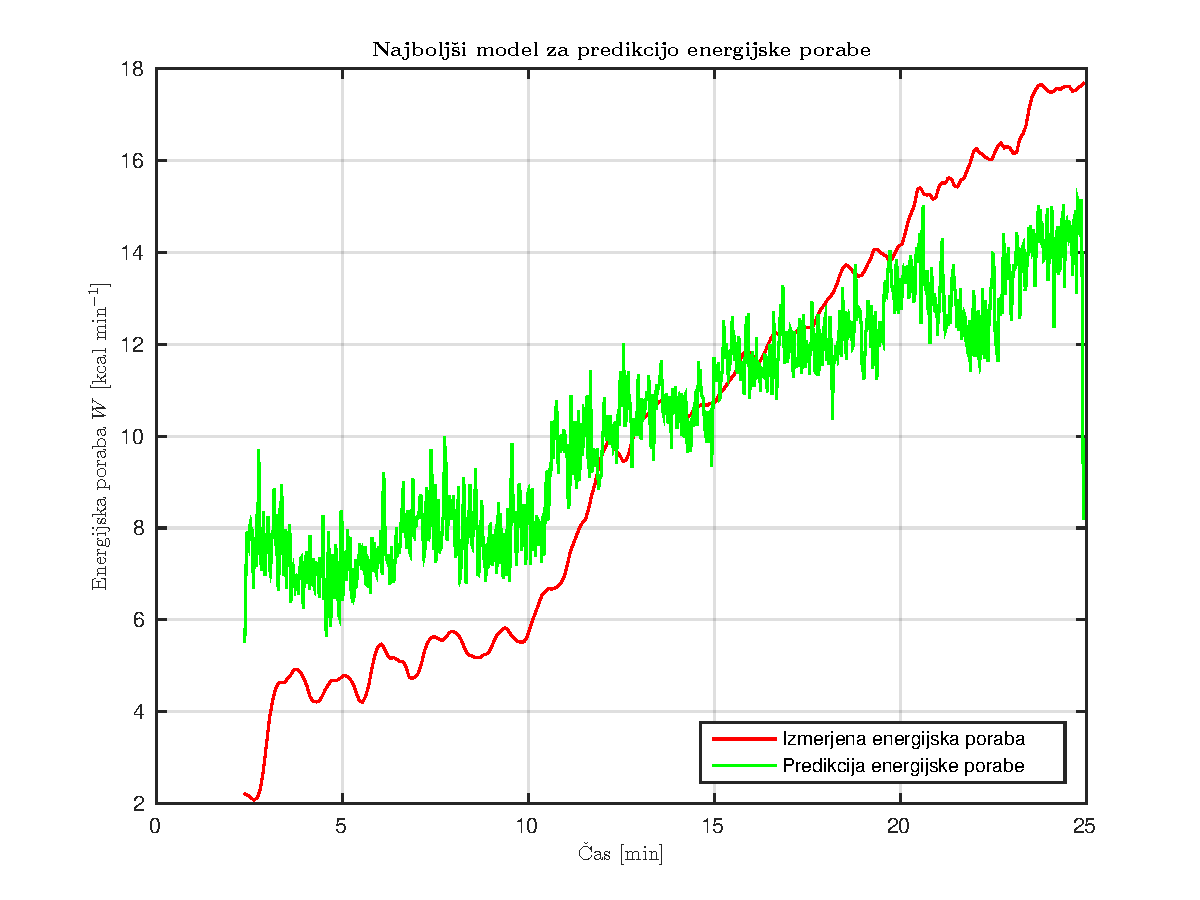
\includegraphics[width=\columnwidth]{best-results-stage3-ff-lab-of-3-subj5-backview-backview-normal-val-sl}
		\caption{Rezultati eem-sv-of-subj9(sv) z optičnim tokom}
		\label{fig:lab-of-3}
	\end{subfigure}
	~
	\begin{subfigure}[t]{0.45\columnwidth}
		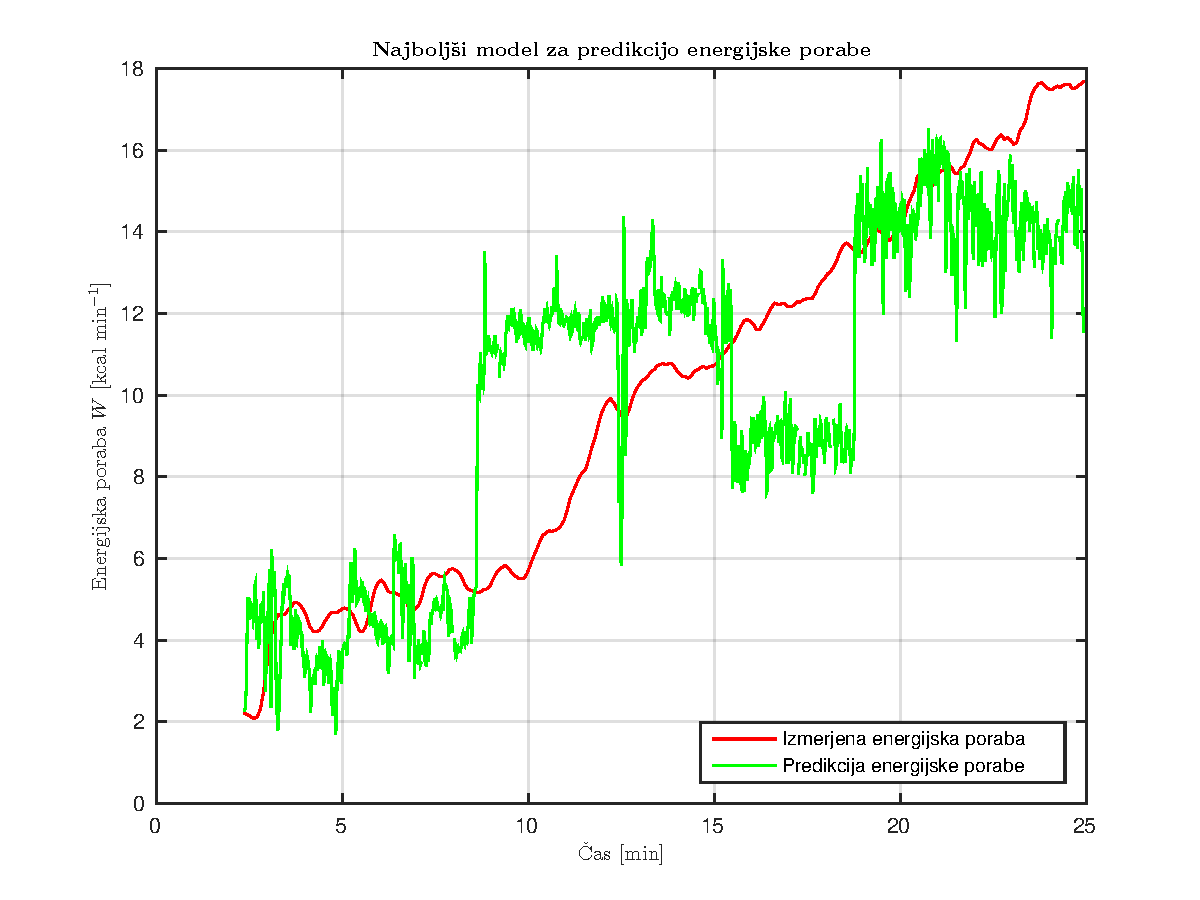
\includegraphics[width=\columnwidth]{best-results-stage3-ff-lab-sf-3-subj5-backview-backview-normal-val-sl}
		\caption{Rezultati eem-sv-sf-subj9(sv) s prostorskim tokom}
		\label{fig:lab-sf-3}
	\end{subfigure}
	\caption[Odziv SUBJ9 modelov protokola 3 druge faze laboratorijskih eksperimentov]{Odziv najboljših modelov protokola 3 druge faze laboratorijskih eksperimentov. Rdeča krivulja predstavlja merjen parameter, zelena predikcijo. Na sliki \subref{fig:lab-of-3}) je najboljši rezultat pri uporabi optičnega toka. Na sliki \subref{fig:lab-sf-3}) je najboljši rezultat pri uporabi prostorskega toka.}
	\label{fig:lab-3}
\end{figure}

\subsection{Terenski eksperimenti}
\subsubsection{Odvisnost na akumulacijo utrujenosti}
V tabeli \ref{tab:stage2-field-1-mean} je predstavljeno povprečje validacij merjencev za protokol 1. Pearsonov korelacijski koeficient (CORR) smo povprečili s Fisherjevo $z$ transformacijo. Najboljše rezultate dobimo za prostorski tok \textit{sf}. Korelacija je dokaj visoka, ampak metrike napak nakazujejo na slabši model.

\begin{table}[!htbp]
	\centering
	\begin{tabular}{l S[table-format=1.2, round-mode=places, round-precision=2] S[table-format=1.2, round-mode=places, round-precision=2] S[table-format=1.2, round-mode=places, round-precision=2] S[table-format=1.2, round-mode=places, round-precision=2]}
		\toprule
		\textbf{Model} & \thead{CORR} & \thead{RAE} & \thead{RRSE} & \thead{nSV} \\
		\midrule
		\tdata{stage2-field-1-mean}
		\bottomrule
	\end{tabular}
	\caption[Povprečje validacij merjencev za protokol 1 2. faze terenskih eksperimentov]{Povprečje validacij merjencev za protokol 1 druge faze terenskih eksperimentov. Pearsonov korelacijski koeficient (CORR) smo povprečili s Fisherjevo $z$ transformacijo.}
	\label{tab:stage2-field-1-mean}
\end{table}

V tabeli \ref{tab:stage2-field-2-mean} predstavljamo povprečje rezultatov za protokol 2. Pearsonov korelacijski koeficient (CORR) smo povprečili s Fisherjevo $z$ transformacijo. Vsi modeli imajo pričakovano nizko korelacijo in veliko napak.

\begin{table}[!htbp]
	\centering
	\begin{tabular}{l S[table-format=1.2, round-mode=places, round-precision=2] S[table-format=1.2, round-mode=places, round-precision=2] S[table-format=1.2, round-mode=places, round-precision=2] S[table-format=1.2, round-mode=places, round-precision=2]}
		\toprule
		\textbf{Model} & \thead{CORR} & \thead{RAE} & \thead{RRSE} & \thead{nSV} \\
		\midrule
		\tdata{stage2-field-2-mean}
		\bottomrule
	\end{tabular}
	\caption[Povprečje validacij merjencev za protokol 2 2. faze terenskih eksperimentov]{Povprečje validacij merjencev za protokol 2 druge faze terenskih eksperimentov. Pearsonov korelacijski koeficient (CORR) smo povprečili s Fisherjevo $z$ transformacijo.}
	\label{tab:stage2-field-2-mean}
\end{table}

\subsubsection{Generalizacija modela}
S protokolom 3 smo želeli preveriti, če lahko uporabimo generaliziran model za predikcijo energijske porabe na različnih merjencih. Rezultati so vidni v tabeli \ref{tab:stage2-field-3}. Tukaj dobimo najboljše rezultate pri uporabi prostorskega toka, kot smo to predlagali tudi sami. Tudi rezultati optičnega toka niso slabi. Najboljši rezultati za optični in prostorski tok, so predstavljeni na sliki \ref{fig:lab-3}.

\begin{table}[!htbp]
	\centering
	\begin{tabular}{l S[table-format=1.2, round-mode=places, round-precision=2] S[table-format=1.2, round-mode=places, round-precision=2] S[table-format=1.2, round-mode=places, round-precision=2] S[table-format=1.2, round-mode=places, round-precision=2]}
		\toprule
		\textbf{Model} & \thead{CORR} & \thead{RAE} & \thead{RRSE} & \thead{nSV} \\
		\midrule
		\tdata{stage2-field-3}
		\bottomrule
	\end{tabular}
	\caption[Validacijske metrike za protokol 3 2. faze terenskih eksperimentov]{Validacijske metrike za protokol 3 druge faze terenskih eksperimentov.}
	\label{tab:stage2-field-3}
\end{table}

\begin{figure}[!htbp]
	\centering
	\begin{subfigure}[t]{0.45\columnwidth}
		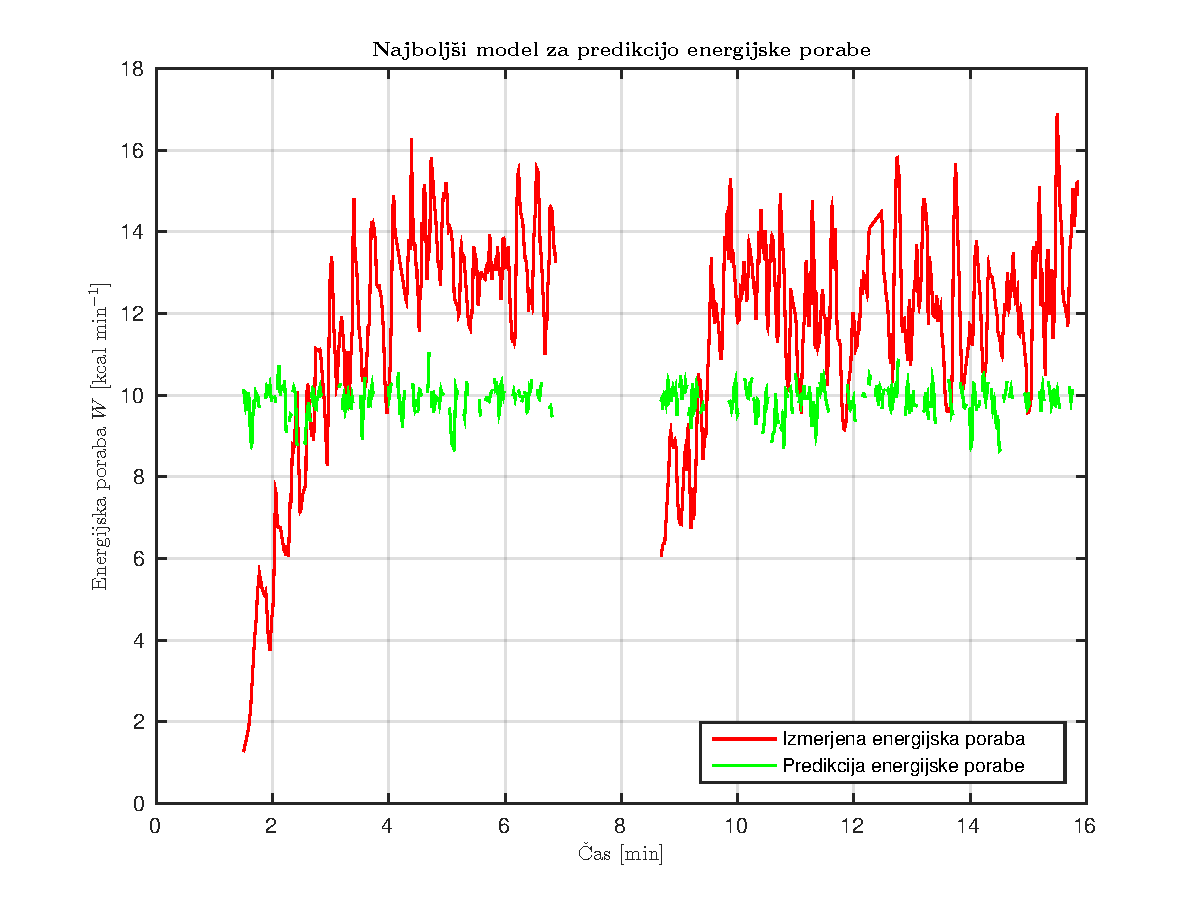
\includegraphics[width=\columnwidth]{best-results-stage3-ff-field-of-3-subj6-backview-backview-normal-val-sl}
		\caption{Rezultati eem-bv-of-subj9(bf) z optičnim tokom}
		\label{fig:field-of-3}
	\end{subfigure}
	~
	\begin{subfigure}[t]{0.45\columnwidth}
		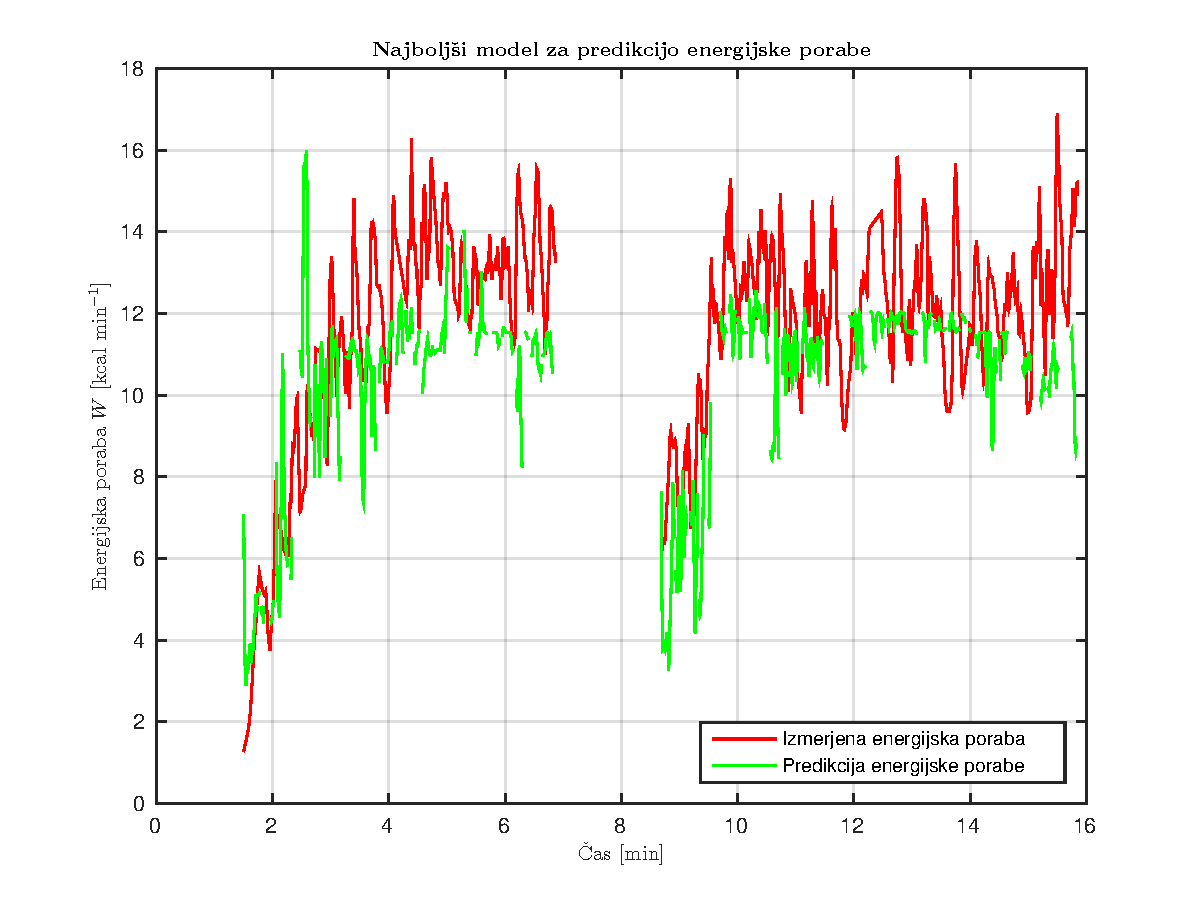
\includegraphics[width=\columnwidth]{best-results-stage3-ff-field-sf-3-subj6-backview-backview-normal-val-sl}
		\caption{Rezultati flow eem-bv-sf-subj9(bv) s prostorskim tokom}
		\label{fig:field-sf-3}
	\end{subfigure}
	\caption[Odziv SUBJ9 modelov protokola 3 2. faze lab. eksperimentov]{Odziv najboljših modelov protokola 3 druge faze laboratorijskih eksperimentov. Rdeča krivulja predstavlja merjen parameter, zelena predikcijo. Na sliki \subref{fig:field-of-3}) je najboljši rezultat pri uporabi optičnega toka. Na sliki \subref{fig:field-sf-3}) je najboljši rezultat pri uporabi prostorskega toka.}
	\label{fig:field-3}
\end{figure}










